\RequirePackage{ifpdf}
\ifpdf
   \documentclass[a4paper,11pt,pdftex,twoside]{scrartcl}
\else
   \documentclass[a4paper,11pt,dvips,twoside]{scrartcl}
\fi

% ------------------------------------------------------------------------------
% Include packages
% ------------------------------------------------------------------------------
\ifpdf
   \usepackage[pdftex]{color}
   \usepackage[final,pdftex]{graphicx} % Einbinden von Gaphiken, flexibler als package {graphics}
\else
   \usepackage[dvips]{color}
   \usepackage[final,dvips]{graphicx}
\fi
\usepackage[english]{babel}
\usepackage[utf8]{inputenc}  % Ermöglicht die Verwendung von UTF8 Zeichensätzen
                             % und damit der direkten Eingabe von "deutschen" Sonderzeichen, d.h. z.B. Umlaute.
\usepackage[T1]{fontenc}
\usepackage{caption}
\usepackage{tabularx}
\usepackage{longtable}
\usepackage{natbib}
\usepackage{booktabs}
\usepackage[table]{xcolor}
\usepackage{xspace}   % \xspace
\usepackage{float}    % {table}[H]
\usepackage{lscape}   % {landscape}
\usepackage[left=2cm,right=2cm,top=1cm,bottom=1cm,includeheadfoot]{geometry}
\usepackage{hyperref}
\usepackage{enumitem}

\hypersetup{
  linktocpage,
  colorlinks=true,
  linkcolor=blue,
}

% PAGE LAYOUT
%\setlength{\topmargin}{-1cm}
%\setlength{\headheight}{0cm}
%\setlength{\headsep}{0cm}
%\setlength{\textheight}{\paperheight}
%\addtolength{\textheight}{-1in}

\setlength{\oddsidemargin}{0.1cm}
\setlength{\evensidemargin}{\oddsidemargin}
\setlength{\textwidth}{\paperwidth}
\addtolength{\textwidth}{-2in}
\addtolength{\textwidth}{-1.8\oddsidemargin}

% new commands
\newcommand{\superscript}[1]{\ensuremath{^{\textrm{#1}}}}
\newcommand{\subscript}[1]{\ensuremath{_{\textrm{#1}}}}

\renewcommand{\th}[0]{\superscript{th}}
\newcommand{\st}[0]{\superscript{st}}
\newcommand{\nd}[0]{\superscript{nd}}
\newcommand{\rd}[0]{\superscript{rd}}

\newcommand{\celsius}{$^{\circ}\mathrm{C}$\xspace}
\newcommand{\degree}{$^{\circ}$\xspace}

\newcommand{\dir}{\emph}
\newcommand{\cmdname}{\emph}

\renewcommand{\bf}{\normalfont \bfseries}

% Color defintions
\definecolor{darkgray}{rgb}{0.85,0.85,0.85}
\definecolor{lightgray}{rgb}{0.95,0.95,0.95}

% alternate rowcolors for all long-tables
%\let\oldlongtable\longtable
%\let\endoldlongtable\endlongtable
%\renewenvironment{longtable}{\rowcolors{2}{darkgray}{lightgray}\oldlongtable} {
%\endoldlongtable}

% ============================================================================
% Define Titlepage
% ============================================================================
%\subject{}
\title{
  \begin{center}
    \vspace{-10mm}
    \rule{0.9\textwidth}{0.5pt}
    \vspace{7mm}
    {\bf \huge Pyrad }\\[10mm]
    {\bf \huge Data Processing Cookbook}\\
    \vspace{-3mm}
    \rule{0.9\textwidth}{0.5pt}
  \end{center}
}
%\author{Andreas Leuenberger}
\date{}
%\publishers{\vspace{20mm}}  % Abused to separate title from abstract
\titlehead{
  \vspace{-10mm}
  \hspace*{0cm}
  
\includegraphics[width=1.0\textwidth]{./figures/titlebar.pdf}\\[20mm]
  \vspace{0mm}
  \hspace{0mm}
}

% ============================================================================

\begin{document}

% ----------------------------------------------------------------------------
% Make titlepage
% ----------------------------------------------------------------------------
\maketitle
\thispagestyle{empty} % No headers, no page numbers
% Include title picture
%\vspace{-20mm}
%\begin{figure}[htbp]
%  \begin{center}
%    \includegraphics[width=0.7\columnwidth]{images/dx50_small}
%    \caption*{Wetterradar DX50}
%  \end{center}
%\end{figure}
%\vspace{20mm}
\vfill
Version: 0.4.0\\
Date: October, 18, 2017
\clearpage

% ----------------------------------------------------------------------------
% Version control page
% ----------------------------------------------------------------------------

\thispagestyle{empty} % No headers, no page numbers

\section*{Document History}

\subsection*{Responsible People}
\begin{table}[H]
\begin{center}
\begin{tabularx}{\textwidth}{|l|X|}
  \hline
  Creation/Edition        & J.~Grazioli\\ \hline
  Revision                & \\  \hline
  Approval                & \\  \hline
  Further information     & Document editors\\  \hline
\end{tabularx}
\end{center}
\end{table}

\subsection*{Versionenkontrolle}
%\begin{tabularx}{\textwidth}{|l|l|l|X|}
\begin{longtable}{|p{0.08\textwidth}|p{0.17\textwidth}|p{0.12\textwidth}|p{0.52\textwidth}|}

  \hline
  {\bf Version} & {\bf Edited by}         & {\bf Date}  & {\bf Activity}\\
  \hline
  \endfirsthead

  \multicolumn{4}{l}%
  {\textit{Continued from previous page}}\\
  \hline
  {\bf Version} & {\bf Edited by}         & {\bf Date}  & {\bf Activity}\\
  \hline
  \endhead

  \hline
  \multicolumn{4}{r}{\textit{Continued on next page}}\\
  \endfoot

  \hline
  \endlastfoot

  0.2.0         & J.~Grazioli    & 2017-08-23  & Creation begun \\ \hline
  0.3.0         & J.~Grazioli    & 2017-10-18  & check products section \\ \hline
  0.4.0         & J.~Grazioli, J.~Figueras i Ventura & 2017-11-28 & Review and structural modification \\ 
  0.5.0         & D.~Wolfensberger & 2021-01-12 & Added section on GECSX \\ 
  
  \hline 
 
\end{longtable}

\clearpage

% ----------------------------------------------------------------------------
% Table of content
% ----------------------------------------------------------------------------

\thispagestyle{empty} % No headers, no page numbers
\tableofcontents
\clearpage


%\pagestyle{plain} % No headers, just page numbers
\pagenumbering{arabic} % Roman numerals
\setcounter{page}{1}   % Start page numbering

% ----------------------------------------------------------------------------
% Introduction
% ----------------------------------------------------------------------------
\section{Introduction}

\subsection{Motivation for Separating Code and Configuration}
\begin{itemize}
  \item A future ''final'' version of the code should not be touched.
  \item Clear change and versioning control of the code.
  \item No local file paths and personal settings in the code.
  \item Developing and test can be done using local config files.
  \item Parameters are not hard coded and can be changed easily.
  \item High flexibility. All settings are made by changing only 1--3
    config files.
\end{itemize}

\subsection{Rationale and other sources of information}
The processing is based on the PyRad framework. \underline{Usually} pyrad is cloned in the home directories of each users in the appropriate servers. As an example, for zueub222 and user jgr:

\begin{verbatim}
jgr@zueub222:pyrad$ pwd
/home/lom/users/jgr/pyrad
\end{verbatim} 

The purpose of this document is to allow users to process data by manipulating only configuration files. The focus is therefore here on the processing output and not on PyRad itself. For an overview of the functionalities of PyRad, its installation, and development, please refer to the documentation available at:

\begin{verbatim}
pyrad/doc/
\end{verbatim}

that includes the following main documents:
\begin{itemize}
   \item {\it pyart-mch\_library\_reference\_dev}:
   \item {\it pyart-mch\_library\_reference\_users}:
\end{itemize}

% ----------------------------------------------------------------------------
% Data Processing
% ----------------------------------------------------------------------------
\newpage
\section{Data Processing}

\subsection{Data Processing}
The information about this section is complementary to Sec.~2 of the document:

\begin{verbatim}
   pyrad/doc/pyrad_user_manual.docx
\end{verbatim}


The data processing can be started from the linux shell, after activation of the proper conda environment. Depending on the server, the appropriate environment may be  ``root'' (i.e. for zueub222):

\begin{verbatim}
jgr@zueub222:~$ source activate root
(root) jgr@zueub222:~$ 
\end{verbatim}

\noindent
or it can be ``pyrad'' (i.e. for CSCS and cirrus servers).
The python scripts used to process the radar data can be called from the directory:

\begin{verbatim}
pyrad/src/pyrad_proc/scripts/
\end{verbatim}

\noindent
The scripts that are useful for this document are the following processing and realtime scripts:
\begin{itemize}
   \item main\_process\_data.py
   \item main\_process\_data\_rt.py
   \item main\_process\_data\_period.py
   \item process\_trajectory.py (obsolete, other functions should be used)
\end{itemize}
they can all be called from the linux shell.

\subsubsection{Process data real time (main\_process\_data\_rt.py)}
This script is designed to process data in real time. It can operate in two different ways:
\begin{itemize}
\item The script is ``listening'' on some data folders and immediately process new data se they appear. The script therefore remains active all the time.
\item The script is periodically restarted by cronjob.
\end{itemize}

Verbatim, from the help page of the script:
\begin{verbatim}
This program performs real time processing of the data

To run the processing framework type:
    python main_process_data.py [config_files] 
     --starttime [process_start_time] --endtime [process_end_time] 
     --cfgpath [cfgpath] --proc_period [proc_period]

If startime or endtime are specified the program will start processing at the
specified time and end at the specified time. Otherwise the program ends when
the user interrupts it.
cfgpath is an optional argument with default: '$HOME/pyrad/config/processing/'
proc_period is the time that has to pass before attempting to restart the
processing in s
if proc_finish is not none it indicates the time the program is allowed to ran
berfore forcing it to end


Example:
    python main_process_data.py 'paradiso_fvj_vol.txt' 'paradiso_fvj_rhi.txt' 
    --starttime '20140523000000' --endtime '20140523001000' 
    --cfgpath '$HOME/pyrad/config/processing/' --proc_period 60 --proc_finish 120


usage: main_process_data_rt.py [-h] [--starttime STARTTIME]
                               [--endtime ENDTIME] [--cfgpath CFGPATH]
                               [--proc_period PROC_PERIOD]
                               [--proc_finish PROC_FINISH]
                               cfgfiles [cfgfiles ...]

Entry to Pyrad processing framework

positional arguments:
  cfgfiles              name of main configuration file

optional arguments:
  -h, --help            show this help message and exit
  --starttime STARTTIME
                        starting time of the data to be processed. Format
                        YYYYMMDDhhmmss
  --endtime ENDTIME     end time of the data to be processed. Format
                        YYYYMMDDhhmmss
  --cfgpath CFGPATH     configuration file path
  --proc_period PROC_PERIOD
                        Period between processing rounds (s)
  --proc_finish PROC_FINISH
                        Processing time allowed before shutdown (s)

\end{verbatim}

\subsubsection{Process data (main\_process\_data.py)}
Standard data processing (i.e., usually non real time) is performed by this script.
Verbatim from the help page:

\begin{verbatim}
This program processes and post-processes data over a time span

To run the processing framework type:
    python main_process_data.py [config_file] --starttime [process_start_time] --endtime
     [process_end_time] --postproc_cfgfile [postproc_config_file] --cfgpath [cfgpath]

If startime and endtime are not specified the program determines them from
the trajectory file or the last processed volume.
postproc_cfgfile is an optional argument with default: None
cfgpath is an optional argument with default: '$HOME/pyrad/config/processing/'

Example:
    python main_process_data.py 'paradiso_fvj_vol.txt' --starttime '20140523000000' 
    --endtime '20140523001000' --postproc_cfgfile 'paradiso_fvj_vol_postproc.txt' --cfgpath
     '$HOME/pyrad/config/processing/'


usage: main_process_data.py [-h] [--starttime STARTTIME] [--endtime ENDTIME]
                            [--postproc_cfgfile POSTPROC_CFGFILE]
                            [--cfgpath CFGPATH] [-i INFOSTR] [-t TRAJFILE]
                            proc_cfgfile

Entry to Pyrad processing framework

positional arguments:
  proc_cfgfile          name of main configuration file

optional arguments:
  -h, --help            show this help message and exit
  --starttime STARTTIME
                        starting time of the data to be processed. Format
                        YYYYMMDDhhmmss
  --endtime ENDTIME     end time of the data to be processed. Format
                        YYYYMMDDhhmmss
  --postproc_cfgfile POSTPROC_CFGFILE
                        name of main post-processing configuration file
  --cfgpath CFGPATH     configuration file path
  -i INFOSTR, --infostr INFOSTR
                        Information string about the actual data processing
                        (e.g. 'RUN57'). This string is added to the filenames
                        of the product files.
  -t TRAJFILE, --trajfile TRAJFILE
                        Definition file of plane trajectory. Configuration of
                        scan sector, products, ...


\end{verbatim}

\subsubsection{Process data (main\_process\_data\_period.py)}
This script is used in post-processing to process data over long periods of time, usually several days.
It can, for example:
\begin{itemize}
   \item Process several individual days.
   \item Process several days portions (e.g. several days, all from 08 to 10)
\end{itemize}

According to its help entry:
\begin{verbatim}
This program does the daily processing and post-processing over a period of time.

To run the processing framework type:
    python main_process_data.py [config_file] [process_start_date] [process_end_date] 
    --starttime [process_start_time] --endtime [process_end_time] --postproc_cfgfile
     [postproc_config_file] --cfgpath [cfgpath]

starttime is an optional argument with default: '000000'
endtime is an optional argument with default: '235959'
postproc_cfgfile is an optional argument with default: None
cfgpath is an optional argument with default: '$HOME/pyrad/config/processing/'

Example:
    python main_process_data.py 'paradiso_fvj_vol.txt' '20140523' '20140525' 
    --starttime '000000' --endtime '001000' --postproc_cfgfile 'mals_emm_vol_postproc.txt' 
    --cfgpath '$HOME/pyrad/config/processing/'


usage: main_process_data_period.py [-h] [--starttime STARTTIME]
                                   [--endtime ENDTIME]
                                   [--postproc_cfgfile POSTPROC_CFGFILE]
                                   [--cfgpath CFGPATH]
                                   proc_cfgfile startdate enddate

Entry to Pyrad processing framework

positional arguments:
  proc_cfgfile          name of main configuration file
  startdate             starting date of the data to be processed. Format
                        YYYYMMDD
  enddate               end date of the data to be processed. Format YYYYMMDD

optional arguments:
  -h, --help            show this help message and exit
  --starttime STARTTIME
                        starting date of the data to be processed. Format
                        hhmmss
  --endtime ENDTIME     end date of the data to be processed. Format hhmmss
  --postproc_cfgfile POSTPROC_CFGFILE
                        name of main post-processing configuration file
  --cfgpath CFGPATH     configuration file path

\end{verbatim}

This script creates the product once all the data has been processed.

\subsubsection{Process trajectories (process\_trajectory.py)}
This script is used in post-processing to process trajectory data. 
The usage of this script is:

\begin{verbatim}
usage: process_trajectory.py [-h] [-c CFGFILE]
                             [--preproc_cfgfile PREPROC_CFGFILE] [-i INFOSTR]
                             trajfile [starttime] [endtime]

Create PYRAD products using a plane trajectory

positional arguments:
  trajfile              Definition file of plane trajectory. Configuration of
                        scan sector, products, ...
  starttime             Starting time of the data to be processed. Format:
                        YYYYMMDDhhmm[ss]. If not given, the time of the first
                        sample is used.
  endtime               End time of the data to be processed. Format:
                        YYYYMMDDhhmm[ss]. If not given, the time of the last
                        sample is used.

optional arguments:
  -h, --help            show this help message and exit
  -c CFGFILE, --cfgfile CFGFILE
                        Main configuration file. Defines the
  --preproc_cfgfile PREPROC_CFGFILE
                        name of main pre-processing configuration file
  -i INFOSTR, --infostr INFOSTR
                        Information string about the actual data processing
                        (e.g. 'RUN57'). This string is added to the filenames
                        of the product files.

Example:
  process_trajectory.py -c $HOME/pyrad/config/processing/mals_emm_rw22_traj.txt
     --preproc_cfgfile $HOME/pyrad/config/processing/mals_emm_rw22_traj_preproc.txt
     -i TS011 /data/mals_plane_traj/EMM/gnv_20161026_ts011_seat_emmen_flt01_ADS.txt

\end{verbatim}

% ----------------------------------------------------------------------------
% Configuration
% ----------------------------------------------------------------------------
\newpage
\section{Configuration}
\label{sec_configuration}

The configuration of the data processing is divided into three files. The
\emph{main configuration file} (see Section~{\ref{subsec_main_config}),
the \emph{location configuration file} (see Section~{\ref{subsec_location_config})
describing the location of the weather radar and the used scans.
The \emph{product configuration file} describes the datasets and products. As this
is bit more complicated it is described in its own Section~{\ref{sec_products}.

The configuration files are located in \dir{malsgit/config\_pyrad/processing/}.




\subsection{Main Configuration File}
\label{subsec_main_config}
Tha main configuration file is used to define the global settings, notably the paths to the different sources of data.
The parameters of the main configuration file are described in
Table~\ref{tab_main_config_params}

\begin{longtable}{p{0.20\textwidth}p{0.10\textwidth}p{0.60\textwidth}}
\caption{Configuration parameters of the main configuration file}\\
\label{tab_main_config_params}

\bf{Name}          & \bf{Type} & \bf{Description}\\
\hline
\endfirsthead

\multicolumn{3}{c}%
{\tablename\ \thetable\ -- \textit{Continued from previous page}}\\
\bf{Name}          & \bf{Type} & \bf{Description}\\
\hline
\endhead

\hline
\multicolumn{3}{r}{\textit{Continued on next page}}\\
\endfoot

\hline
\endlastfoot

name               & STRING    & Name of the data processing. This name is used
                                 in the path of the saved products in the following manner:
                                 <saveimgbasepath>/<name>/<YYYY-MM-DD>/<datasetname>/<prodname>/
                                 <outputname>\\
datapath           & STRING    & Base directory of the rainbow raw data. This field
                                 must have a trailing '/'. The raw data files of a scan
                                 can be found using the following file path:\\
                   &           & <datapath>/<scanname>/<YYYY-MM-DD>/<YYYYMMDDHHMMSS00datatype>.<ext>\\
configpath         & STRING    & Base directory of the configuration files. This directory
                                 contains clutter maps, filter coefficients, antenna pattern,
                                 and the data processing configuration files.\\
cosmopath          & STRING    & Base directory of the COSMO data files.\\
dempath            & STRING    & Base directory of the Digital Elevation Model (DEM) files.
                                 Basically to load the radar visibility (Optional)\\
smnpath            & STRING    & Base directory of the SwissMetNet stations data. Used in the
                                 comparison between radar data and rain gauges (Optional)\\
disdropath         & STRING    & Base directory of the disdrometer data. Used in the comparison
                                 between radar data and disdrometers (Optional)\\
solarfluxpath      & STRING    & Base directory of the solar flux data. Used to plot the calibration
                                 bias based on sun monitoring (Optional)\\
locationConfigFile & STRING    & File name (with full path) of the location configuration file.\\
                   &           & Described in Section~\ref{subsec_location_config}.\\
productConfigFile  & STRING    & File name (with full path) of the product configuration file.\\
                   &           & Described in Section~\ref{sec_products}.\\
lastStateFile      & STRING    & File name (with full path) of the file containing the time
                                 of the last processed scan. Used in particular for real time
                                  processing.\\
imgformat          & STRING/STRARR  & File format(s) of the images. The following formats are supported:
                                 eps, png and jpg. If \emph{saveimg} is set to 0, this field is
                                 not used.\\
saveimgbasepath    & STRING    & Base directory for the images to save. The directory structure
                                 looks as follows:
                                 <saveimgbasepath>/<name>/<YYYY-MM-DD>/<datasetname>/<prodname>/
                                 <outputname>
                                 If \emph{saveimg} is set to 0, this field is not used.\\
loadbasepath       & STRING    & OPTIONAL. Base path of saved data. By default, this field is set to
                                 \emph{saveimgbasepath}.\\
loadname           & STRING    & OPTIONAL. Name of the saved data processing. Used for saved volume loading.
                                 By default, this field is set to \emph{name}.\\
\end{longtable}

\subsection{Location Configuration File}
\label{subsec_location_config}

The location configuration files describes some parameters that are depending on the specific location of a radar (type of scans we want to measure, radar name, etc ). The location of the weather
radar (its position) itself, is instead usually read from the radar metadata directly and it is not necessarily defined in this file.
The fields are described in Table~\ref{tab_location_config_params}.

\begin{longtable}{p{0.23\textwidth}p{0.10\textwidth}p{0.57\textwidth}}
\caption{Configuration parameters of the location configuration file}\\
\label{tab_location_config_params}
\bf{Name}          & \bf{Type} & \bf{Description}\\
\hline
\endfirsthead

\multicolumn{3}{c}%
{\tablename\ \thetable\ -- \textit{Continued from previous page}}\\
\bf{Name}          & \bf{Type} & \bf{Description}\\
\hline
\endhead

\hline
\multicolumn{3}{r}{\textit{Continued on next page}}\\
\endfoot

\hline
\endlastfoot

RadarName      & STRING    & Short version name of a C-band radar (i.e. A, D, L, P) or DX50, MXPol for the X-band radars.\\
RadarRes      & STRING    & rad4alp radar resolution (H or L). Only necessary if rad4alp data is processed\\

RadarBeamwidth & FLOAT & Radar antenna beam width [Deg]\\
AntennaGaindB & FLOAT & antenna gain [dB]\\
ScanList           & STRARR    & A list with the scans used for this data processing.
                                 Note that the first scan in this list is used as master scan.
                                 The master scan must be the first (temporal) scan of the
                                 corresponding rainbow task. In case of composite volumes the master scan is usually a PPI and the following are RHIs. If the radar processed is MCH C-band the scan list consists of the radar elevation (i.e. from 001 to 020).\\
                   &           & All scan names must have a trailing '/' except if rad4alp data is processed\\
%compose\_volume    & INT       & Boolean (defaul 0/NO). If 1, the volumes of the ScanList are composed to form a COMPOSITE\_VOLUME dataset (See~\ref{subsec_composite_volume_dataset})\\
ScanPeriod         & FLOAT     & Repetition period of each scan in minutes.\\
Azimtol            & FLOAT     & Tolerance in azimuth for irregular data. (0.5 is a good value)\\
clutterMap         & STRING    & Clutter map of the data processing. The clutter map is
                                 located at <configpath>/clutter/<clutterMap>\\
AntennaGain        & FLOAT & Radar antenna gain. Not used for X-band MCH data. \\ 
radarconsth(v)        & FLOAT & Radar constant h (v). Not mandatory. \\
mflossh(v)            & Matched filter losses h (v). Not mandatory. \\
attg                & FLOAT & Gas attenuation coeafficient ({\bf units?} (1 way attenuation) \\                                
CosmoRunFreq & INT &  Frequency of a COSMO model run in hours.\\
CosmoForecasted & INT & Hours forecasted by the COSMO model.\\
rmax            & FLOAT & For C-band data, the maximum range in [m] to be considered. USeful for speed
                                 considerations.   \\
elmax           & FLOAT & Maximum elevation [$^\circ$] to consider  \\                                 
ppiImageConfig     & STRUCT    & Structure defining the PPI image generating. The following 6
                                 fields are described below:\\
rhiImageConfig     & STRUCT    & Structure defining the RHI image generating. The following 6
                                 fields are described below:\\
$\quad$ xsize      & INT       & Number of horizontal pixels of the picture (without frame).\\
$\quad$ ysize      & INT       & Number of vertical pixels of the picture (without frame).\\
$\quad$ xmin       & FLOAT     & Distance of the left image boundary to the radar in km.\\
$\quad$ xmax       & FLOAT     & Distance of the right image boundary to the radar in km.\\
$\quad$ ymin       & FLOAT     & Distance of the lower image boundary to the radar in km.\\
$\quad$ ymax       & FLOAT     & Distance of the upper image boundary to the radar in km.\\

ppiMapImageConfig     & STRUCT & Structure defining the PPI image overlayed on a map. The following 9 fields are described below:\\
$\quad$ rngRing  & FLOAT      & Distance between range rings (0 means no range ring) [km].\\
$\quad$ xsize    & FLOAT      & Image size (inches) [ich].\\
$\quad$ ysize    & FLOAT      & Image size [ich].\\
$\quad$ lonmin   & FLOAT      & Minimum WGS84 longitude [$^\circ$].\\
$\quad$ lonmax   & FLOAT      & Maximum WGS84 longitude [$^\circ$].\\
$\quad$ latmin   & FLOAT      & Minimum WGS84 latitude [$^\circ$].\\
$\quad$ latmax   & FLOAT      & Maximum WGS84 latitude [$^\circ$].\\
$\quad$ mapres   & STRING     & Map resolution. Accepted strings are: ``10m'', ``50m'', ``110m'' \\
$\quad$ maps     & STRARR     & String array of possible maps to overplot. Accepted entries include: 
                                relief, countries, provinces, urban\_areas, roads, railroads, 
                                coastline, lakes, lakes\_europe, rivers, rivers\_europe   \\



rvsazImageConfig     & STRUCT    & Structure defining the range versus azimuth image. The following 4 fields are described below:\\
$\quad$ xmin       & FLOAT     & Min angle on horizontal axis [Deg].\\
$\quad$ xmax       & FLOAT     & Max angle on horizontal axis [Deg].\\
$\quad$ ymin       & FLOAT     & Min range on vertical axis [km].\\
$\quad$ ymax       & FLOAT     & Max range on vertical axis [km].\\

rvselImageConfig     & STRUCT    & Structure defining the range versus elevation image. It contains the same 4 fields as rvsazImageConfig.\\

sunhitsImageConfig     & STRUCT    & Structure defining the sun hits image. The following 6 fields are described below:\\
$\quad$ xsize      & INT      & Number of horizontal pixels of the picture (without frame).\\
$\quad$ ysize      & INT    & Number of vertical pixels of the picture (without frame).\\
$\quad$ xmin      & FLOAT  & Minimum azimuth angle difference (between sun and radar).\\
$\quad$ xmax     & FLOAT  & Maximum azimuth angle difference (between sun and radar).\\
$\quad$ ymin      & FLOAT  & Minimum elevation angle difference (between sun and radar).\\
$\quad$ ymax     & FLOAT  & Maximum azimuth angle difference (between sun and radar).\\


$\quad$ azPatternFile & STRING & Name of the azimuth pattern file of the antenna. This file and
                                 path must be
                                 <configpath>/antenna/<azPatternFile>\\
$\quad$ elPatternFile & STRING & Name of the elevation pattern file of the antenna. This file and
                                 path must be
                                 <configpath>/antenna/<elPatternFile>\\
$\quad$ fixed\_angle  & FLOAT  & Fixed angle of a PAR antenna in degrees. For the PAR azimuth
                                 antenna this is the elevation angle. For the elevation antenna
                                 is is the azimuth angle.\\
\end{longtable}


\newpage

% ----------------------------------------------------------------------------
% Product Generation Configuration
% ----------------------------------------------------------------------------
\section{Product Generation Configuration}
\label{sec_products}

This section describes the product configuration.

\subsection{Basic Concept}

The concept is based on three stages: 1. input or raw data volume, 2. datasets
and 3. products.

The center point of the data processing is the dataset. A dataset can be
generated from one or more than one input data volumes (e.g. a rainrate dataset
uses 5 different raw data volume to be generated).

There are several different formats of a dataset. For example, a dataset can be a
volume, a trajectory, a volume composite or a time series.
Section~\ref{sec_datasets} summarizes the possible datasets.

From a dataset the products are generated. What products can be generated from
a dataset depends on the type (volume, volume composite, trajectory or
time series) of the dataset.

Figure~\ref{fig_main_concept} shows a schema of an example of the basic concept
of the product generation. From different input data a dataset
is generated and from this dataset m products are created.

\begin{figure}[htbp]
  \begin{center}
    \ifpdf
      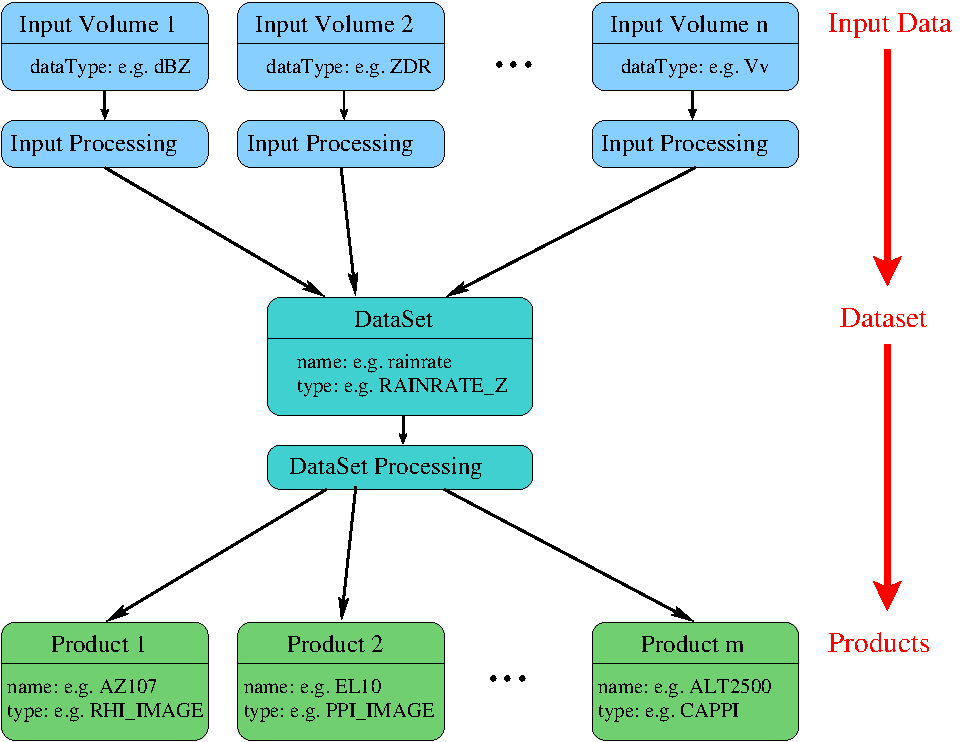
\includegraphics[width=0.9\textwidth]{./figures/main_concept.pdf}
    \else
      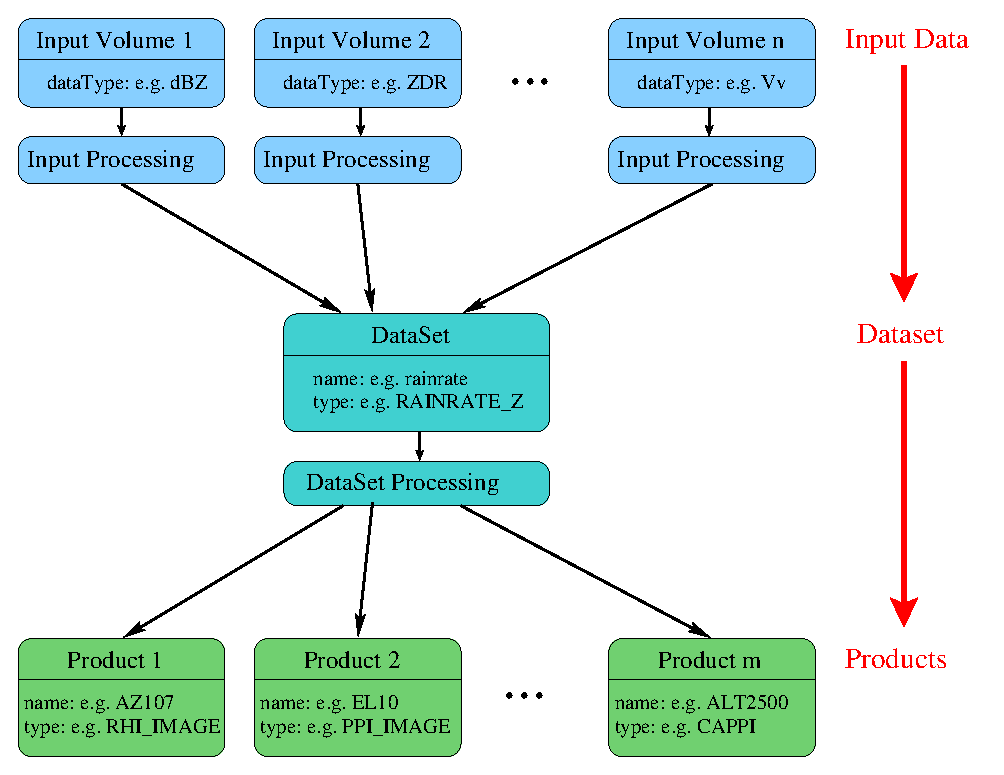
\includegraphics[width=0.9\textwidth]{./figures/main_concept.eps}
    \fi
  \end{center}
  \caption{Basic concept for product generation from input (also called raw) data.}
  \label{fig_main_concept}
\end{figure}

The dataset types are described in Section~\ref{sec_datasets}
and the product types in Section~\ref{sub_products}





\subsection{Input Volume Datatypes}

There are different group of input volume datatypes that can be read as input data
for a dataset. These groups are summarized in Table~\ref{tab_datatype_groups}. The possible volume datatypes for each datatype group are listed in Table~\ref{tab_datatypes}.

The specification of the datatype for a dataset is done by first writing the datatype
group, followed by a ':' and then the name of the datatype. If no ':' is given, it is
assumed that the datatype belongs to the group \emph{RAW}.
For a datatype from the group \emph{SAVED}, the dataset and product name must be
specified. This information is separated by ','.
Note that \emph{NETCDF} datatypes cannot be mixed with other datatypes.\\

\noindent
{\bf Caveat:} please do not mistake the input volume datatype with the dataset type (entry  ``type'' of the dataset structure)
\begin{verbatim}
<datasetname> STRUCT 2
   type     STRING <datasettype>
   datatype STRARR
      RAW:dBZ
      PSR:NhDBM
      COSMO:TEMP
      SAVED:RR_h,<olddataset>,<oldproduct>
\end{verbatim}

\begin{table}[H]
\rowcolors{1}{darkgray}{lightgray}
\begin{tabularx}{\textwidth}{lX}
\bf{Group} & \bf{Description}\\
RAW       & Raw data generated by the DX50 (or other rainbow format). Stored in rainbow data format.\\
CFRADIAL     & A dataset generated by this dataprocessing procedure. As additional
            information the dataset and the product name of the previous dataset
            must be specified.\\
COSMO     & Data created by COSMO. Converted to polar radar coordinates and
            stored in rainbow file format.\\
DEM     & Digital Elevation Model data (DEM). Basically visibility in rainbow file format\\
NETCDF    & {\bf NOT THERE YET!} \\

RAD4ALP & rad4alp data.\\
RAD4ALPDEM & rad4alp visibility data.\\
RAD4ALPCOSMO & a binary file with COSMO data for rad4alp processing.\\
PROC & indicates that the dataset is the result of the preprocessing of raw data. (i.e. it will be created on the fly).\\

\end{tabularx}
\caption{List of input volume datatype groups}
\label{tab_datatype_groups}
\end{table}


\begin{table}[H]
\rowcolors{1}{darkgray}{lightgray}
\begin{tabularx}{\textwidth}{lX}
\bf{Group} & \bf{Datatypes}\\
\hline
RAW      & dBZ, dBZv, dBuZ, dBuZv, V, Vv, Vu, Vvu, W, Wv, Wu, Wvu,
            KDP, uKDP, uKDPu, PhiDP, uPhiDP, uPhiDPu, RhoHV,
            RhoHVu, uRhoHV, L, ZDR, ZDRu, SQI, SQIv, SQIu, SQIvu, SNRh, SNRv, CDR\\
IQ        & Same as PSR plus WhADU, WvADU, WhDBADU, WvDBADU, WhDBM, WvDBM, WhDBZ, WvDBZ, IhCPX, IvCPX, IhRAW, IvRAW, IhADU, IvADU, IhDBADU, IvDBADU, IhDBM, IvDBM, IhDBZ, IvDBZ, IhDEG, IvDEG\\
CFRADIAL     & (Some examples, not complete) dV, dVv, dVu, dVvu, RR\_Zh, RR\_Ah,
            RR\_Kdp, Att, SAN, TRAJ, HEIGHT, WP, WPDIFF, WPRELDIFF,
            dtfilter, RAINEXT, RCS\\
COSMO     & ISO0, TEMP, H\_ISO0\\
DEM         & VIS\\
NETCDF    & {\bf NICE TO HAVE, NOT THERE YET} \\
RAD4ALP & dBZ, ZDR, RhoHV, uPhiDP, V, W, SNRh, SNRv, L, CDR.\\
RAD4ALPDEM & VIS.\\
RAD4ALPCOSMO & ISO0, TEMP\\
PROC & dBZc, dBZvc, ZDRc, PhiDPc, KDPc, RhoHVc, Ah, Adp.\\
\end{tabularx}
\caption{List of possible datatypes}
\label{tab_datatypes}
\end{table}


\subsection{Product Configuration File}

The product configuration files describes the products that are generated
for the data processing. The fields are described in
Table~\ref{tab_product_config_params}.

\begin{longtable}{p{0.20\textwidth}p{0.10\textwidth}p{0.60\textwidth}}
\caption{Configuration parameters of the product configuration file}\\
\label{tab_product_config_params}
\bf{Name}          & \bf{Type} & \bf{Description}\\
\hline
\endfirsthead

\multicolumn{3}{c}%
{\tablename\ \thetable\ -- \textit{Continued from previous page}}\\
\bf{Name}          & \bf{Type} & \bf{Description}\\
\hline
\endhead

\hline
\multicolumn{3}{r}{\textit{Continued on next page}}\\
\endfoot

\hline
\endlastfoot

dataSetList        & STRARR    & A list of the datasets that are generated for the
                                 data processing. There must be a structure in the product
                                 configuration file defining
                                 the dataset and its product for each dataset in
                                 this list. The list of datasets may include the processing level.
                                 {\bf TODO: add link to the definition of processing level}   \\
<datasetname>      & STRUCT    & A structure defining a dataset. The <datasetname> must
                                 be a member of the \emph{dataSetList} list. The structure
                                 defines the type of the dataset, its parameters and the
                                 products that are applied to this dataset.
                                 The <datasetname> can be freely chosen. Just make sure the
                                 spelling is the same in the dataSetList.
                                 The <datasetname> is used for the path to store the
                                 products:
                                 <saveimgbasepath>/<name>/<YYYY-MM-DD>/<datasetname>/<prodname>/
                                 <outputname>.\\
                   &           & The mandatory fields of this structure are described below.
                                 The fields depending on the dataset type are described in
                                 Section~\ref{sec_datasets}.\\
\hangindent=1em \hangafter=0
type               & STRING    & Type of the dataset. The tables in Section~\ref{sec_datasets} list
                                 all possible dataset types.\\
\hangindent=1em \hangafter=0
datatype           & STRARR    & Raw (or input) datatype. The dataset is generated using
                                 rainbow raw files of this datatypes or the dataset is
                                 generated using multiple raw files with different datatypes.\\
\hangindent=1em \hangafter=0
IGNORE\_\-MISSING\_VOLS & INT & OPTIONAL. If set, the function processing the dataset
                                 is called if not all input data volumes could be selected. For
                                 example this could be used for the sanity check. In such a case
                                 only the checks are done with the available input volumes.
                                 By default, this option is off. {\bf TODO: can be removed?}\\
\hangindent=1em \hangafter=0
        DSSAVENAME & STRING   &  OPTIONAL. Usually the product files are stored under the name of the
                                 dataset. If this parameter is saved, the files are stored under
                                 this name instead of the dataset name.\\
\hangindent=1em \hangafter=0
        INPUT\-PROCESSING & STRUCT & OPTIONAL. Input processing of one or more input volumes. See
                                 section~\ref{subsec_general_processing} for details. {\bf TODO: can be removed?}\\
\hangindent=1em \hangafter=0
        DATASET\-PROCESSING & STRUCT & OPTIONAL. Dataset processing of a volume dataset. See
                                 section~\ref{subsec_general_processing} for details. {\bf TODO: can be removed?}\\
\hangindent=1em \hangafter=0
        products   & STRUCT    & This structure contains a list of products. Each product
                                 is a structure named as <prodname>. For the product
                                 description see Section~\ref{sub_products}.\\
\hangindent=2em \hangafter=0
        <prodname> & STRUCT    & Structure defining a product of the dataset.
                                 The <prodname> can be freely chosen. The <prodname> is
                                 used to store the output products:
                                 <saveimgbasepath>/<name>/<YYYY-MM-DD>/<datasetname>/<prodname>/
                                 <outputname>.\\
                   &           & The mandatory fields of this structure are described below.
                                 The fields depending on the product type are described in
                                 Section~\ref{sub_products}.\\
\hangindent=2.1em \hangafter=0
         type      & STRING    & Type of the product. Section~\ref{sub_products} describes all possible
                                 product types.\\
\end{longtable}

\paragraph{Example:} A simple product config file is listed below:
\begin{verbatim}
#
# Product generation configuration
#

# List of datasets to generate.
# The detailed specification of each dataset is given below.
dataSetList STRARR 12
   l0:TEMP
   l0:reflectivity
   l0:ZDR
   l0:RhoHV   
   l0:echoID
   l1:echoFilter
   l3:echoFilter_Ah
   l2:outlierFilter
   l2:Att_ZPhi
   l3:hydroclass
   l4:rainrate   
   l3:wind


# ==========================================================================================
#               COSMO data
# ==========================================================================================
TEMP STRUCT 6
    type STRING COSMO_LOOKUP
    datatype STRARR 1
        dBZ        
    cosmo_type STRING TEMP
    regular_grid INT 0
    lookup_table INT 1
    MAKE_GLOBAL INT 1
	
	
# ==========================================================================================
#                 raw data processing
# ==========================================================================================
reflectivity STRUCT 3
   type     STRING RAW
   datatype STRING dBZ
   products STRUCT 4      
      EL03_0 STRUCT 3
         type  STRING PPI_IMAGE
         anglenr INT 0
         voltype STRING dBZ
      EL04_0 STRUCT 3
         type  STRING PPI_IMAGE
         anglenr INT 1
         voltype STRING dBZ
      EL05_7 STRUCT 3
         type  STRING PPI_IMAGE
         anglenr INT 2
         voltype STRING dBZ      
      SAVESTATE STRUCT 2
         type STRING SAVESTATE
         voltype STRING dBZ
         
ZDR STRUCT 3
   type     STRING RAW
   datatype STRING ZDR
   products STRUCT 3      
      EL03_0 STRUCT 3
         type  STRING PPI_IMAGE
         anglenr INT 0
         voltype STRING ZDR
      EL04_0 STRUCT 3
         type  STRING PPI_IMAGE
         anglenr INT 1
         voltype STRING ZDR
      EL05_7 STRUCT 3
         type  STRING PPI_IMAGE
         anglenr INT 2
         voltype STRING ZDR
         
RhoHV STRUCT 3
   type     STRING RAW
   datatype STRING RhoHV
   products STRUCT 3      
      EL03_0 STRUCT 3
         type  STRING PPI_IMAGE
         anglenr INT 0
         voltype STRING RhoHV
      EL04_0 STRUCT 3
         type  STRING PPI_IMAGE
         anglenr INT 1
         voltype STRING RhoHV
      EL05_7 STRUCT 3
         type  STRING PPI_IMAGE
         anglenr INT 2
         voltype STRING RhoHV
		 
		 
# ==========================================================================================
#                 echo identification
# ==========================================================================================
echoID STRUCT 3
    type STRING SAN
    datatype STRARR 4
        dBZ
        ZDR
        uPhiDP
        RhoHV
    MAKE_GLOBAL INT 1


# ==========================================================================================
#                 clutter and noise suppression
# ==========================================================================================
# echo type 3 : precip, 2 : clutter, 1 : noise
echoFilter STRUCT 4
    type STRING ECHO_FILTER
    datatype STRARR 8
        PROC:echoID
        dBZ        
        ZDR
        RhoHV
        PhiDP
        KDP
		V
		W
    echo_type INT 3
    MAKE_GLOBAL INT 1

echoFilter_Ah STRUCT 4
    type STRING ECHO_FILTER
    datatype STRARR 2
        PROC:echoID
        PROC:Ah
    echo_type INT 3
    MAKE_GLOBAL INT 1
	
	
# ==========================================================================================
#                 outlier filter
# ==========================================================================================    
outlierFilter STRUCT 8
    type STRING OUTLIER_FILTER
    datatype STRARR 1
        PROC:Vc
    threshold FLOAT 10.
    nb INT 2
    nb_min INT 3
    percentile_min FLOAT 5.
    percentile_max float 95.
    MAKE_GLOBAL INT 1


# ==========================================================================================
#                 Attenuation
# ==========================================================================================
Att_ZPhi STRUCT 5
    type STRING ATTENUATION
    datatype STRARR 4
        PROC:dBZc
        PROC:ZDRc
        PROC:PhiDPc
        PROC:TEMP
    ATT_METHOD STRING ZPhi
    fzl FLOAT 2000.
    MAKE_GLOBAL INT 1

	
# ==========================================================================================
#                 hydrometeor classification products
# ==========================================================================================
hydroclass STRUCT 5
    type STRING HYDROCLASS
    datatype STRARR 5
        PROC:dBZc
        PROC:ZDRc
        PROC:RhoHVc
        PROC:KDPc
        PROC:TEMP
    HYDRO_METHOD STRING SEMISUPERVISED
    RADARCENTROIDS STRING DX50
    MAKE_GLOBAL INT 1


# ==========================================================================================
#               rainfall rate
# ==========================================================================================            
rainrate STRUCT 5
    type STRING RAINRATE
    datatype STRARR 3
        PROC:dBZc
        PROC:Ahc
        PROC:hydro
    RR_METHOD STRING hydro
    MAKE_GLOBAL INT 1
    products STRUCT 3      
      EL03_0 STRUCT 3
         type  STRING PPI_IMAGE
         anglenr INT 0
         voltype STRING RR
      EL04_0 STRUCT 3
         type  STRING PPI_IMAGE
         anglenr INT 1
         voltype STRING RR
      EL05_7 STRUCT 3
         type  STRING PPI_IMAGE
         anglenr INT 2
         voltype STRING RR

			
# ==========================================================================================
#               wind velocity
# ==========================================================================================
wind STRUCT 5
    type STRING WIND_VEL
    datatype STRARR 1
        PROC:Vc
    vert_proj INT 0
    MAKE_GLOBAL INT 1
    products STRUCT 3      
      EL03_0 STRUCT 3
         type  STRING PPI_IMAGE
         anglenr INT 0
         voltype STRING wind_vel_h_az
      EL04_0 STRUCT 3
         type  STRING PPI_IMAGE
         anglenr INT 1
         voltype STRING wind_vel_h_az
      EL05_7 STRUCT 3
         type  STRING PPI_IMAGE
         anglenr INT 2
         voltype STRING wind_vel_h_az
\end{verbatim}

The example product configuration files defines twelve datasets: let us take the example of \emph{l0:reflectivity}
and \emph{l4: rainrate}.

The \emph{reflectivity} dataset is a \emph{RAW} dataset generated using the raw
datatype \emph{dBZ}. Four products are generated for this dataset: the products
\emph{EL03\_0}, \emph{EL04\_0}, \emph{EL05\_7} which are of type \emph{PPI\_IMAGE} (the first, second and third PPIs in a volume scan, as given in field \emph{anglenr}). The images are stored in
<saveimgbasepath>/<name>/<YYYY-MM-DD>/reflectivity/EL0X\_X/. The fourth product saves the volume in the path given by \emph{loadbasepath} fo the main configuration file. 

The \emph{rainrate} dataset is a \emph{RAINRATE} dataset generated using the processed
datatypes \emph{dBZc}, \emph{Ahc}, \emph{hydro}, by means of the \emph{HYDRO} retrieval method.
In analogous way with respect to the \emph{reflectivity} dataset, PPI images are generated as products.

\subsection{The concept of processing level}

Processing level(s) are defined in the product configuration file, in  the initial definition of the dataset list (i.e. $l0$, $l1$, $l2$\dots). The processing level defines the order in which the datasets
will be processed. This is particularly useful when subsequent processing levels need data from previous datasets. In this case, the order matters, and the option ``MAKE\_GLOBAL'' should be used. 

\newpage

% ---------------------------------------------------------------------------------
% Datasets
% ---------------------------------------------------------------------------------
\section{Datasets}
\label{sec_datasets}
A thorough description of the available datasets can be found in Sec.~2 of {\bf pyrad\_library\_reference\_user}. The dataset type is defined by the ``type'' entry in the 
dataset block of the product configuration file. Dataset types can be found in Table~\ref{tab_datasets_type}. 

%\begin{table}[H]
%\rowcolors{1}{darkgray}{lightgray}
%\begin{tabularx}{\textwidth}{lXl}
%{\bf Name} & {\bf Description} & {\bf Reference}\\
\subsection{Dataset type and format}

 The field ``type'', for each dataset listed in the product configuration, takes the values as in
Table~\ref{tab_datasets_type}. Depending on the type, the proper pyrad/pyart processing routine is 
applied. Each dataset type has a dataset ``format'' (more types may correspond to the same format),
that will be used to generate the appropriate products.


\begin{longtable}{p{0.40\textwidth}p{0.40\textwidth}p{0.10\textwidth}}
\caption{List of dataset types with basic identification.}\\
\label{tab_datasets_type}
\bf{Type}          & \bf{(Format) Explanation} & \bf{Reference}\\
\hline
\endfirsthead

\multicolumn{3}{c}%
{\tablename\ \thetable\ -- \textit{Continued from previous page}}\\
\bf{Name}          & \bf{Type} & \bf{Reference}\\
\hline
\endhead

\hline
\multicolumn{3}{r}{\textit{Continued on next page}}\\
\endfoot

\hline
\endlastfoot

RAW & (VOL) Process raw data &  \\
GRID & (GRID) Grid data & \\
QVP & (QVP) Quasi-Vertical-Profile & \\
TIME\_HEIGHT & (QVP) Time-height time series & \\
CDF & (VOL)  Cumulative Density Function & \\
NCVOL & (VOL) Volume in NetCDF format & \\
PWR & (VOL) Signal power & \\
SNR & (VOL) Signal-to-noise ratio & \\
RHOHV\_CORRECTION & (VOL) Noise correction $\rho_{HV}$ & \\
BIAS\_CORRECTION & (VOL) Bias correction & \\
L & (VOL) &  \\
CDR & (VOL) & \\
SAN & (VOL) Echo identification/sanity & \\
CLT\_TO\_SAN & (VOL) Clutter to echo classification & \\
ECHO\_FILTER & (VOL)   Filter on echo classification & \\
SNR\_FILTER & (VOL) Filter on SNR & \\
VIS\_FILTER & (VOL) Filter on visibility & \\
OUTLIER\_FILTER & (VOL) Filter outliers & \\
PHIDP0\_CORRECTION & (VOL) Correct on starting $\Phi_{dp}$ & \\
PHIDP\_SMOOTH\_1w & (VOL) Single window wmoothing of $\Phi_{dp}$ & \\
PHIDP\_SMOOTH\_2w & (VOL) Double window wmoothing of $\Phi_{dp}$ & \\
PHIDP\_KDP\_VULPIANI & (VOL) $\Phi_{dp}$ and $K_{dp}$ estimation by Vulpiani et al. & \\
PHIDP\_KDP\_KALMAN & (VOL) $\Phi_{dp}$ and $K_{dp}$ estimation by Schneebeli et al. & \\
PHIDP\_KDP\_MAESAKA & (VOL) $\Phi_{dp}$ and $K_{dp}$ estimation by Maesaka et al. & \\
PHIDP\_KDP\_LP & (VOL) $\Phi_{dp}$ and $K_{dp}$ estimation by ?? & \\
KDP\_LEASTSQUARE\_1W & (VOL) $K_{dp}$ estimation, single window least square & \\
KDP\_LEASTSQUARE\_2W & (VOL) $K_{dp}$ estimation, double window least square & \\
ATTENUATION & (VOL) Radar attenuation & \\
RAINRATE & (VOL) Rainrate estimation & \\
WIND\_VEL & (VOL) Wind velocity (radial) estimation & \\
WINDSHEAR & (VOL) Wind shear (spectral width) & \\
HYDROCLASS & (VOL) Hydrometeor identification & \\
ML\_DETECTION &  (VOL) Melting layer detection & \\
PHIDP0\_ESTIMATE &  (VOL) Estimation of $\Phi_{dp0}$ & \\
RHOHV\_RAIN & (VOL) $\rho_{hv}$ in rain & \\
ZDR\_PREC &  (VOL) $Z_{DR}$ in precipitation& \\
ZDR\_SNOW &  (VOL) $Z_{DR}$ in  snow & \\
SELFCONSISTENCY\_KDP\_PHIDP & (VOL) Self consistency & \\
SELFCONSISTENCY\_BIAS & (VOL) Bias from consistency & \\
COSMO & (VOL) COSMO data & \\
COSMO\_LOOKUP & (VOL) Cosmo lookup table & \\
COSMO\_COORD & (COSMO\_COORD) Cosmo coordinates & \\
HZT\_LOOKUP & (VOL) HZT lookup table & \\
HZT  & (VOL) & \\ 
TIME\_AVG & (TIMEAVG) Time averaging & \\
FLAG\_TIME\_AVG & (TIMEAVG) Time average flag& \\
COLOCATED\_GATES & (COLOCATED\_GATES) Process colocated gates of radars & \\
INTERCOMP & (INTERCOMP) Radars intercomparison & \\
INTERCOMP\_TIME\_AVG & (INTERCOMP) Time average intercomparison& \\
MONITORING & (MONITORING) Data monitoring & \\
GC\_MONITORING & (MONITORING) Data monitoring ?? & \\
OCCURRENCE & (OCCURRENCE) & \\
OCCURRENCE\_PERIOD & (OCCURRENCE) & \\
SUN\_HITS & (SUN\_HITS) Sun hits in radar data & \\
POINT\_MEASUREMENT & (TIMESERIES) & \\
TIMESERIES & (TIMESERIES) Time series & \\
TRAJ & (TRAJ\_ONLY) Trajectory & \\
TRAJ\_ATPLANE & (TIMESERIES) Trajectory at plane/object location & \\
TRAJ\_ANTENNA\_PATTERN & (TIMESERIES) Trajectory at plane/object location, given antenna pattern & \\
TRAJ\_LIGHTNING & (TIMESERIES) Trajectory at lighning locations & \\

\end{longtable}

%\end{tabularx}
%\caption{List of all possible dataset types.}
%\label{tab_datasets_type}
%\end{table}


\subsection{Datasets and configuration parameters}

{\bf TODO TODO}






\newpage

% ---------------------------------------------------------------------------------
% Products
% ---------------------------------------------------------------------------------
\section{Products}
\label{sub_products}

For each dataset format several products can be generated, as seen in the product generation file.
The list of products for each dataset are passed as a string array, and each product is defined as a structure.
Different product ``type'' can be selected, determining the subsequent process.
Not all product types are available for each data type. 
The following tables and sections list the possible products for each dataset format.


\subsection{VOL products}
Listed here are the products for VOL dataset formats.

\begin{table}[H]
\rowcolors{1}{darkgray}{lightgray}
\begin{tabularx}{\textwidth}{lXl}
{\bf Name}      & {\bf Description}                      & {\bf Reference} \\
PPI\_IMAGE      & PPI image of constant elevation        &  {Sec:~\ref{subsec_ppi_image}} \\
PPI\_MAP        & PPI image on a map                     &  {Sec:~\ref{subsec_ppi_map}}    \\
PSEUDOPPI\_IMAGE  & Reconstructed PPI from non-PPI data  &  {Sec:~\ref{subsec_pseudoppi_image}}   \\
PSEUDOPPI\_MAP  & PSEUDO-PPI on a map                 &  {Sec: ~\ref{subsec_pseudoppi_map}} \\
RHI\_IMAGE      & RHI image of constant azimuth          & Sec: ~\ref{subsec_rhi_image}   \\
RHI\_PROFILE    & Averaged height profile                & Sec: ~\ref{subsec_rhi_profile} \\
PSEUDORHI\_IMAGE   &                 & Sec: ~\ref{subsec_pseudorhi_image}    \\
CAPPI\_IMAGE        & Constant altitude PPI image            &  Sec: ~\ref{subsec_cappi_image}   \\
PLOT\_ALONG\_COORD & Plot along coordinates                 & Sec: ~\ref{subsec_plot_along_coord}  \\
BSCOPE\_IMAGE & B-scope type image (ray versus range)    &  Sec: ~\ref{subsec_bscope_image} \\
TIME\_RANGE & Time vs range display                 &  Sec: ~\ref{subsec_time_range}  \\
HISTOGRAM & Histogram of the variable               &  Sec: ~\ref{subsec_histogram}  \\
QUANTILES & Quantiles of some variables               & Sec: ~\ref{subsec_quantiles}  \\
FIELD\_COVERAGE &                & Sec: ~\ref{subsec_field_coverage}  \\
CDF & Cumulative density function  & Sec: ~\ref{subsec_cdf}  \\
SAVEVOL         & Save the generated dataset volume        & Sec: ~\ref{subsec_savevol}  \\
SAVEALL & {\bf TODO: describe}                 & Sec: ~\ref{subsec_saveall}  \\
SAVESTATE       & Save the time of the processed volume. & Sec: ~\ref{subsec_savestate} \\
\end{tabularx}
\caption{List of all possible product types for dataset VOL format}
\label{tab_products_VOL}
\end{table}


\subsubsection{PPI\_IMAGE}
   \label{subsec_ppi_image}

 PPI image of constant elevation.
The parameters of a \emph{PPI\_IMAGE} product are listed in Table~\ref{tab_product_ppi_image}.

\begin{table}[H]
 \rowcolors{1}{darkgray}{lightgray}
 \begin{tabularx}{\textwidth}{llX}
 \bf{Parameter}  & \bf{Type}  & \bf{Description}\\
 TYPE           & STRING     & Must be \emph{PPI\_IMAGE}.\\
 anglenr        & INT        & Elevation number (starting with 0) of the PPI image
                               to generate.\\
 voltype        & STRING     &  A valid datatype string (i.e., KDP, KDPc, TYPE, dBZ\dots)\\

 \end{tabularx}
 \caption{Parameters of a PPI\_IMAGE product.}
 \label{tab_product_ppi_image}
\end{table}
 The dimension and boundaries of the PPI image are set in the location configuration file (Sec.~\ref{subsec_location_config}).

\subsubsection{PPI\_MAP}
   \label{subsec_ppi_map}

 PPI image of constant elevation on a map
The parameters of a \emph{PPI\_MAP} product are the same as listed in Table~\ref{tab_product_ppi_image}.
 The dimension and boundaries of the PPI map are set in the location configuration file (Sec.~\ref{subsec_location_config}).
 
 
 \subsubsection{PSEUDOPPI\_IMAGE}
    \label{subsec_pseudoppi_image}
Pseudo-PPI is a PPI reconstruction from volumic data (they can be also a series of RHIs), not from genuine PPIs. 
It is displayed as a PPI. The parameters of a PSEUDOPPI\_IMAGE can be found in Table~\ref{tab_product_pseudoppi_image}.

\begin{table}[H]
 \rowcolors{1}{darkgray}{lightgray}
 \begin{tabularx}{\textwidth}{llX}
 \bf{Parameter}  & \bf{Type}  & \bf{Description}\\
 TYPE           & STRING     & Must be \emph{PSEUDOPPI\_IMAGE}.\\
 angle          & FLOAT      & Elevation angle, in degrees of the pseudo-PPI \\
 voltype        & STRING     & A valid datatype string (i.e., KDP, KDPc, TYPE, dBZ\dots)\\
 EleTol         & FLOAT      & Elevation tolerance on the given angle, in degrees. \\
 \end{tabularx}
 \caption{Parameters of a PSEUDOPPI\_IMAGE product.}
 \label{tab_product_pseudoppi_image}
\end{table}

\subsubsection{PSEUDOPPI\_MAP}
   \label{subsec_pseudoppi_map}
As for Sec.~\ref{subsec_pseudoppi_image}, but displayed on a map. 

\subsubsection*{RHI\_IMAGE}
   \label{subsec_rhi_image}
RHI image of constant azimuth.
The parameters of a \emph{RHI\_IMAGE} product are listed in Table~\ref{tab_product_rhi_image}.

\begin{table}[H]
 \rowcolors{1}{darkgray}{lightgray}
 \begin{tabularx}{\textwidth}{llX}
 \bf{Parameter}  & \bf{Type}  & \bf{Description}\\
 TYPE           & STRING     & Must be \emph{RHI\_IMAGE}.\\
 anglenr        & INT        & Azimuth number (starting with 0) of the RHI image
                               to generate.\\
 voltype        & STRING     &  A valid datatype string (i.e., KDP, KDPc, TYPE, dBZ\dots)\\

 \end{tabularx}
 \caption{Parameters of a RHI\_IMAGE product.}
 \label{tab_product_ppi_image}
\end{table}
 The dimension and boundaries of the RHI image are set in the location configuration file (Sec.~\ref{subsec_location_config}).



\subsubsection{PSEUDORHI\_IMAGE}
    \label{subsec_pseudorhi_image}
Pseudo-RHI is a PPI reconstruction from volumic data, not from genuine RHIs. 
It is displayed as a PPI. The parameters of a PSEUDORHI\_IMAGE can be found in Table~~\ref{tab_product_pseudorhi_image}.

\begin{table}[H]
 \rowcolors{1}{darkgray}{lightgray}
 \begin{tabularx}{\textwidth}{llX}
 \bf{Parameter}  & \bf{Type}  & \bf{Description}\\
 TYPE           & STRING     & Must be \emph{PSEUDORHI\_IMAGE}.\\
 angle          & FLOAT      & Azimuth angle, in degrees of the pseudo-RHI \\
 voltype        & STRING     & A valid datatype string (i.e., KDP, KDPc, TYPE, dBZ\dots)\\
 EleTol         & FLOAT      & Azimuth tolerance on the given angle, in degrees. \\
 \end{tabularx}
 \caption{Parameters of a PSEUDORHI\_IMAGE product.}
 \label{tab_product_pseudorhi_image}
\end{table}



 \subsubsection{RHI\_PROFILE}
 \label{subsec_rhi_profile}

Averaged height profile. The dataset is limited by the  \emph{rangeStart} and
 \emph{rangeStop} parameters. For each radar gate the vertical height is calculated,
 the heights are divided into height layers. For each height layer the median, the
 15\% and 75\% quantiles are calculated.

The product is a figure data value vs. altitude with median  and the two
 quantile curves. Also a text file with the height profile is
 generated. The height resolution in the text file is according the parameter
 \emph{heightResolution}. In the image file the height resolution is always
 100~m. The height is given in meters above sea level.

The parameters of a \emph{RHI\_PROFILE} product are listed in Table~\ref{tab_product_rhi_profile}.

\begin{table}[H]
 \rowcolors{1}{darkgray}{lightgray}
 \begin{tabularx}{\textwidth}{llX}
 \bf{Parameter}  & \bf{Type}  & \bf{Description}\\
 TYPE           & STRING     & Must be \emph{RHI\_PROFILE}.\\
 anglenr        & INT        & Azimuth number (starting with 0) of the RHI image
                               to generate.\\
 rangeStart     & FLOAT      & Minimal distance to the radar for the gates to be used for the
                               RHI\_PROFILE processing. Given in meters.\\
 rangeStop      & FLOAT      & Maximal distance to the radar for the gates to be used for the
                               RHI\_PROFILE processing. Given in meters.\\
 heightResolution & FLOAT    & Resolution of the height layers for the processing. Is only
                               applied to the text output file. The profile image height
                               resolution is fixed to 100~m.\\
 heightMax & FLOAT    & Maximum height to consider, in [m].\\   
  voltype        & STRING     & A valid datatype string (i.e., KDP, KDPc, TYPE, dBZ\dots)\\
                           
 \end{tabularx}
 \caption{Parameters of a RHI\_PROFILE product.}
 \label{tab_product_rhi_profile}
 \end{table}

 \subsubsection{CAPPI\_IMAGE}
 \label{subsec_cappi_image}

The parameters of a \emph{CAPPI\_IMAGE} product are listed in Table~\ref{tab_product_cappi}.

 \begin{table}[H]
 \rowcolors{1}{darkgray}{lightgray}
 \begin{tabularx}{\textwidth}{llX}
 \bf{Parameter}  & \bf{Type}  & \bf{Description}\\
 TYPE           & STRING     & Must be \emph{CAPPI\_IMAGE}.\\
  voltype        & STRING     & A valid datatype string (i.e., KDP, KDPc, TYPE, dBZ\dots)\\
 altitude       & FLOAT      & Altitude of the CAPPI. In meters above see level.\\
 \end{tabularx}
 \caption{Parameters of a CAPPI product.}
 \label{tab_product_cappi}
 \end{table}

\subsubsection{PLOT\_ALONG\_COORD}
  \label{subsec_plot_along_coord}
Plotting along a given coordinate. The parameters of a PLOT\_ALONG\_COORD product are listed in Table~\ref{tab_product_plot_along_coord}.

\begin{table}[H]
 \rowcolors{1}{darkgray}{lightgray}
 \begin{tabularx}{\textwidth}{llX}
 \bf{Parameter}  & \bf{Type}  & \bf{Description}\\
 TYPE           & STRING     & Must be \emph{PLOT\_ALONG\_COORD}.\\
 voltype        & STRING     & A valid datatype string (i.e., KDP, KDPc, TYPE, dBZ\dots)\\
 mode           & STRING     & \emph{ALONG\_RNG}, or \emph{ALONG\_AZI}, or \emph{ALONG\_ELE}. It sets the radar dimension along which to plot. \\
 fix\_azimuths & FLTARR & All fixed azuth angles (same length of a given second dimension) \\
 fix\_elevations & FLTARR & All fixed elevation angles. \\ 
 fix\_ranges & FLTARR &  All fixed ranges in meters. \\
 AngTol & FLOAT & Tolerance on the angles, in degrees. \\
 value\_start & FLOAT & Starting value of the extracted profile. Units depend on selected ``mode'' \\
 value\_end   & FLOAT & Ending value of the extracted profile. Units depend on selected ``mode''\\
 \end{tabularx}
 \caption{Parameters of a PLOT\_ALONG\_COORD product.}
 \label{tab_product_plot_along_coord}
 \end{table}

If for, example we are interested in extracting data along range (i.e. a radial), we will set the mode as \emph{ALONG\_RNG}, and we will provide the given couples of fixed elevations and azimuths (we will not provide fixed ranges). 

 \subsubsection{BSCOPE\_IMAGE}
 \label{subsec_bscope_image}

The parameters of a \emph{BSCOPE\_IMAGE} product are listed in Table~\ref{tab_product_bscope_image}.
A B-scope is the typical 2D radar display given by ray vs range.

 \begin{table}[H]
 \rowcolors{1}{darkgray}{lightgray}
 \begin{tabularx}{\textwidth}{llX}
 \bf{Parameter}  & \bf{Type}  & \bf{Description}\\
 TYPE           & STRING     & Must be \emph{BSCOPE\_IMAGE}.\\
  voltype        & STRING     & A valid datatype string (i.e., KDP, KDPc, TYPE, dBZ\dots)\\
 anglenr        & INT        & Azimuth number (starting with 0) or elevation number (starting with 0)
                               to generate.\\
 \end{tabularx}
 \caption{Parameters of a radar BSCOPE product.}
 \label{tab_product_bscope_image}
 \end{table}

\subsubsection{TIME\_RANGE}
   \label{subsec_time_range}
Time vs range radar image from volume data. The parameters are given in Table~\ref{tab_product_time_range}. Somehow similar to a BSCOPE.

 \begin{table}[H]
 \rowcolors{1}{darkgray}{lightgray}
 \begin{tabularx}{\textwidth}{llX}
 \bf{Parameter}  & \bf{Type}  & \bf{Description}\\
 TYPE           & STRING     & Must be \emph{TIME\_RANGE}.\\
  voltype       & STRING     & A valid datatype string (i.e., KDP, KDPc, TYPE, dBZ\dots)\\
 anglenr        & INT        & Azimuth number (starting with 0) or elevation number (starting with 0)
                               to generate.\\
 \end{tabularx}
 \caption{Parameters of a radar TIME\_RANGE product.}
 \label{tab_product_time_range}
 \end{table}

\subsubsection{HISTOGRAM}
   \label{subsec_histogram}
   Histogram of VOL data. The HISTOGRAM product accept the following parameters:

\begin{table}[H]
 \rowcolors{1}{darkgray}{lightgray}
 \begin{tabularx}{\textwidth}{llX}
 \bf{Parameter}  & \bf{Type}  & \bf{Description}\\
 TYPE           & STRING     & Must be \emph{TIME\_RANGE}.\\
 voltype       & STRING     & A valid datatype string (i.e., KDP, KDPc, TYPE, dBZ\dots)\\
 anglenr        & INT        & Azimuth number (starting with 0) or elevation number (starting with 0)
                               to generate.\\
 \end{tabularx}
 \caption{Parameters of a radar HISTOGRAM product.}
 \label{tab_product_histogram}
 \end{table}
 
\subsubsection{QUANTILES}
   \label{subsec_quantiles}
Generate quantiles of volume data, for a given variable type. The parameters of a QUANTILE product can be found in Table~\ref{tab_product_quantiles}   
   
   
\begin{table}[H]
 \rowcolors{1}{darkgray}{lightgray}
 \begin{tabularx}{\textwidth}{llX}
 \bf{Parameter}  & \bf{Type}  & \bf{Description}\\
 TYPE           & STRING     & Must be \emph{QUANTILES}.\\
 voltype        & STRING     & Type of volume (i.e., KDP, KDPc, TYPE, dBZ\dots)\\
 quantiles      & FLTARR     & List of quantiles to compute. Example: 50 (50\%, median).\\
 \end{tabularx}
 \caption{Parameters of a radar QUANTILES product.}
 \label{tab_product_quantiles}
 \end{table}   
    
    
\subsubsection{FIELD\_COVERAGE}
   \label{subsec_field_coverage}
Field coverage (for eaxample rain extension) of a given volume type. For its configuration, please see Table~\ref{tab_product_quantiles}   
   
   
\begin{table}[H]
 \rowcolors{1}{darkgray}{lightgray}
 \begin{tabularx}{\textwidth}{llX}
 \bf{Parameter}  & \bf{Type}  & \bf{Description}\\
 TYPE           & STRING      & Must be \emph{FIELD\_COVERAGE}.\\
 voltype        & STRING      & Type of volume (i.e., KDP, KDPc, TYPE, dBZ\dots)\\
 threshold      & FLOAT       & To be given. Threshold on the chosen variable to discriminate its field.\\
 nvalid\_min & FLOAT &  Default: 5. Minimum number of valid points.\\
 ele\_res & FLOAT &  Default: 1. Elevation resolution to be used, in degrees.\\
 azi\_res & FLOAT &  Default: 2. Azimuth resolution to be used, in degrees.\\
 ele\_min & FLOAT &  Default: 0. Minimum elevation angle to use, in degrees.\\
 ele\_max & FLOAT &  Default: 30.Maximum elevation angle to use, in degrees.\\
 ele\_step & FLOAT &  Default: 5. Elevation step to use, in degrees.\\
 ele\_sec\_start & FLOAT & degrees \\
 ele\_sec\_stop & FLOAT &  degrees \\
 quantiles & FLTARR & Quantiles to be considered. \\
 \end{tabularx}
 \caption{Parameters of a radar FIELD\_COVERAGE product.}
 \label{tab_product_field_coverage}
 \end{table}   
        
\subsubsection{CDF}
   \label{subsec_cdf}
Cumulative density function, whose parameters are listed in  Table~\ref{tab_product_cdf}.   
   
\begin{table}[H]
 \rowcolors{1}{darkgray}{lightgray}
 \begin{tabularx}{\textwidth}{llX}
 \bf{Parameter}  & \bf{Type}  & \bf{Description}\\
 TYPE           & STRING      & Must be \emph{CDF}.\\
 voltype        & STRING      & Type of volume (i.e., KDP, KDPc, TYPE, dBZ\dots)\\
 sector         & STRUCT      & If givem a structure used to limit the domain. It includes the fields:    \emph{rmin, rmax, azmin,azmax, elmin, elmax, hmin, hmax}. Also only some of those can be given. \\
 vismin        & FLOAT & \\
 absolute      & INT   & Boolean.  \\
 quantiles     & FLTARR & List of quantiles to be used \\
 use\_nans     & INT  & Boolean. Default False \\
 nan\_value    & FLOAT & Default is 0. Value for NaN data \\
 filterclt   & INT & Boolean. Default is 0 (false). Filter clutter or not. \\
 filterprec  & INTARR & ???\\
  \end{tabularx}
 \caption{Parameters of a radar CDF product.}
 \label{tab_product_cdf}
 \end{table}       
 
 \subsubsection{SAVEVOL}
 \label{subsec_savevol}

Save the generated dataset volume in NetCDF cfradial. The \emph{TRAJ\_SAVED} datasets
 read the saved files and combine them with trajectory data.
The parameters of a \emph{SAVEVOL} product are listed in Table~\ref{tab_product_savevol}.

\begin{table}[H]
 \rowcolors{1}{darkgray}{lightgray}
 \begin{tabularx}{\textwidth}{llX}
 \bf{Parameter}  & \bf{Type}  & \bf{Description}\\
 TYPE           & STRING     & Must be \emph{SAVEVOL}.\\
 \end{tabularx}
 \caption{Parameters of a SAVEVOL product.}
 \label{tab_product_savevol}
 \end{table}

\subsubsection{SAVESTATE}
 \label{subsec_savestate}

Save the time of the processed volume. This is used for the realtime processing.
 The time is written to the file defined by the config parameter \emph{lastStateFile}.

Use this product only for one dataset and only for the realtime processing.
 Because the time is written the same file independently of the dataset. Thus, the previous
 time can be easily overwritten if not paying attenuation.

The parameters of a \emph{SAVESTATE} product are listed in Table~\ref{tab_product_savestate}.

\begin{table}[H]
 \rowcolors{1}{darkgray}{lightgray}
 \begin{tabularx}{\textwidth}{llX}
 \bf{Parameter}  & \bf{Type}  & \bf{Description}\\
 TYPE           & STRING     & Must be \emph{SAVESTATE}.\\
 \end{tabularx}
 \caption{Parameters of a SAVESTATE product.}
 \label{tab_product_savestate}
 \end{table}

\subsubsection{SAVEALL}
   \label{subsec_saveall}
SAVEALL is similar to SAVEVOL.


%% \subsubsection{PLOT\_LINES}
%% \label{subsec_plot_lines}

%% Make a plot the data of the volume as a function of one polar volume
%% parameter (either range, azimuth or elevation) setting the other two
%% parameters to a fixed value.

%% The parameters of a \emph{PLOT\_LINES} product are listed in Table~\ref{tab_product_plot_lines}.

%% \begin{table}[H]
%% \rowcolors{1}{darkgray}{lightgray}
%% \begin{tabularx}{\textwidth}{llX}
%% \bf{Parameter}  & \bf{Type}  & \bf{Description}\\
%% TYPE           & STRING     & Must be \emph{PLOT\_LINES}.\\
%% MODE           & STRING     & Mode of the line plotting. Either \emph{ALONG\_R}
%%                               for plotting the values along the range holding
%%                               the azimuth and elevation angles fixed or \emph{ALONG\_AZ}
%%                               or \emph{ALONG\_EL}.\\
%% FIX\_AZ\_ANGLES & FLTARR    & Value of the fixed azimuth angle in degree. Used in the
%%                               \emph{ALONG\_R} and \emph{ALONG\_EL} mode. If more
%%                               than one angle is given, more than one line is plotted.
%%                               Note that the necessary fixed parameters must have the same length.\\
%% FIX\_EL\_ANGLES & FLTARR    & Value of the fixed elevation angle in degree. Used in the
%%                               \emph{ALONG\_R} and \emph{ALONG\_AZ} mode.\\
%% FIX\_RANGES     & FLTARR    & Value of the fixed range in km. Used in the
%%                               \emph{ALONG\_EL} and \emph{ALONG\_AZ} mode.\\
%% START\_VALUE   & FLOAT      & [Optional] Start value of the running parameter. For mode
%%                               \emph{ALONG\_R} it is a range value in km, for \emph{ALONG\_AZ}
%%                               an azimuth angle in degree and for \emph{ALONG\_EL} an elevation
%%                               angle in degree. If not
%%                               set, the full available parameter range is plotted.\\
%% STOP\_VALUE    & FLOAT      & [Optional] End value of the running parameter.\\
%% COLORS         & STRARR     & [Optional] Color code for the lines. The first entry
%%                               defines the color of the first line. Format:
%%                               Hex code as string with two characters for blue, two for
%%                               green and two for red. Example: '0000ff' is red.\\
%% CFGINFO        & STRING     & Additional information about the product. This
%%                               string is appended to the output files.\\
%% \end{tabularx}
%% \caption{Parameters of a PLOT\_LINES product.}
%% \label{tab_product_plot_lines}
%% \end{table}

%% \subsubsection{CDF\_STAT}
%% \label{subsec_cdf_stat}

%% Cumulative distribution function of the values within a dataset. The cdf is plotted
%% as image and the quantiles (10, 20, 30, 40, 50, 60, 70, 80, 90 and 95\%) are
%% written to a file.

%% Some outliers are removed before calculating the cdf.

%% The parameters of a \emph{CDF\_STAT} product are listed in Table~\ref{tab_product_cdf_stat}.

%% \begin{table}[H]
%% \rowcolors{1}{darkgray}{lightgray}
%% \begin{tabularx}{\textwidth}{llX}
%% \bf{Parameter}  & \bf{Type}  & \bf{Description}\\
%% TYPE           & STRING     & Must be \emph{CDF\_STAT}.\\
%% CFGINFO        & STRING     & Additional information about the product. This
%%                               string is appended to the output files.\\
%% use\_nans      & INT        & If set to 1, all gate value with Nan are set
%%                               to the value given by the \emph{nan\_value} field.
%%                               If set to 0, the NaN gates are not used for the
%%                               cdf calculation.\\
%% nan\_value     & FLOAT      & The gates with NaN are set to this number. If
%%                               \emph{use\_nans} is set to zero, this parameter
%%                               is not used.\\
%% absolute       & INT        & If set to 1, the absolute value of the gate values
%%                               is taken and the cdf of the positive number is calculated.\\
%% sector         & STRUCT     & Structure defining the volume sector boundaries where the
%%                               gates are used the cdf calculation. This structure contains the
%%                               following 8 fields:\\
%% $\quad$ rangeStart& FLOAT   & Minimal distance from radar in meters.\\
%% $\quad$ rangeStop & FLOAT   & Maximal distance from radar in meters.\\
%% $\quad$ azStart   & FLOAT   & Start azimuth angle in degrees.\\
%% $\quad$ azStop    & FLOAT   & End azimuth angle in degrees.\\
%% $\quad$ elStart   & FLOAT   & Start elevation angle in degrees.\\
%% $\quad$ elStop    & FLOAT   & End elevation angle in degrees.\\
%% $\quad$ hmin      & FLOAT   & Minimal height above the radar in meters.\\
%% $\quad$ hmax      & FLOAT   & Maximal height above the radar in meters. If this value is negative,
%%                               the maximal height is the zero degree altitude (ISO0) read from the
%%                               COSMO analysis or forecast.\\
%% \end{tabularx}
%% \caption{Parameters of a CDF\_STAT product.}
%% \label{tab_product_cdf_stat}
%% \end{table}





%% \subsubsection{NETCDF\_CONV}
%% \label{subsec_netcdf_conv}

%% Conversion into single netcdf rhi or ppi slices.

%% The parameters of a \emph{NETCDF\_CONV} product are listed in
%% Table~\ref{tab_product_netcdf_conv}.

%% \begin{table}[H]
%% \rowcolors{1}{darkgray}{lightgray}
%% \begin{tabularx}{\textwidth}{llX}
%% \bf{Parameter}  & \bf{Type}  & \bf{Description}\\
%% TYPE           & STRING     & Must be \emph{NETCDF\_CONV}.\\
%% \end{tabularx}
%% \caption{Parameters of a NETCDF\_CONV product.}
%% \label{tab_product_netcdf_conv}
%% \end{table}

%% \subsubsection{MELTLAYER\_IMAGE}
%% \label{subsec_meltlayer_image}
%% Azimuth-Height graphic indicating the density of points suspected to belong to the melting layer, the altitude of the ISO0 and the retrieved top and bottom of the melting layer.

%% \subsubsection{MELTLAYER\_TS}
%% \label{subsec_meltlayer_ts}
%% Time series plot with two subfigures. The top subfigure plots the evolution of the averaged (in azimuth) of the ISO0 and its standard deviation and the averaged (in azimuth) melting layer top and its standard deviation. The bottom subfigure plots the averaged (in azimuth) evolution of the melting layer thickness and its standard deviation.

%% \subsubsection{SAVE\_DEM}
%% \label{subsec_SAVE_DEM}

%% Save the PPI data of the given volume in a digital elevation model (DEM)
%% file format.

%% The parameters of a \emph{SAVE\_DEM} product are listed in
%% Table~\ref{tab_product_SAVE_DEM}.

%% \begin{table}[H]
%% \rowcolors{1}{darkgray}{lightgray}
%% \begin{tabularx}{\textwidth}{llX}
%% \bf{Parameter}  & \bf{Type}  & \bf{Description}\\
%% TYPE           & STRING   & Must be \emph{SAVE\_DEM}.\\
%% ANGLENR        & INT      & PPI selection from volume. Number of the PPI in the
%%                             volume.\\
%% XCOORDMIN      & FLOAT    & Specify the most West coordinates to be saved.
%%                             Must be the CH1903 coordinate in [m].\\
%% YCOORDMIN      & FLOAT    & Specify the most South coordinates to be saved.
%%                             Must be the CH1903 coordinate in [m].\\
%% XRESOLUTION    & FLOAT    & Resolution in meter to be saved.\\
%% NUM\_X\_SAMPLES & INT     & Number of samples in West-East direction.\\
%% NUM\_Y\_SAMPLES & INT     & Number of samples in South -North direction.\\
%% TITLE          & STRING   & Text to be added to the data file.\\
%% SET\_NANS       & INT     & If set to 1, the Nans are replaced by the value specified
%%                             by the config paramter NAN\_VALUE.\\
%% NAN\_VALUE      & FLOAT   & Value to set the nan values if SET\_NANS is set.\\
%% \end{tabularx}
%% \caption{Parameters of a SAVE\_DEM product.}
%% \label{tab_product_SAVE_DEM}
%% \end{table}

%% \subsubsection{RNGVSANG\_IMAGE}
%% \label{subsec_rngvsang}
%% Create and angle-range color plot for a particular elevation or azimuth given by anglenr according to the string FIXEDANGLE (AZIM or ELEV). If there is only one azimuth angle in the volume, it creates a profile. The function makes use of the structures rvsazImageConfig and rvselImageConfig defined in the location configuration file to set the limits of the plot.

%% \subsubsection{SAVESLICE\_PPI\_ASCII}
%% \label{subsec_SAVESLICE_PPI_ASCII}
%% XXX to be described

%% \subsubsection{CONST\_RANGE\_IMAGE}
%% \label{subsec_CONST_RANGE_IMAGE}

%% Make an azimuth vs. elevation image at given range.

%% The parameters of a \emph{CONST\_RANGE\_IMAGE} product are listed in
%% Table~\ref{tab_product_CONST_RANGE_IMAGE}.

%% \begin{table}[H]
%% \rowcolors{1}{darkgray}{lightgray}
%% \begin{tabularx}{\textwidth}{llX}
%% \bf{Parameter}  & \bf{Type}  & \bf{Description}\\
%% TYPE            & STRING     & Must be \emph{CONST\_RANGE\_IMAGE}.\\
%% RANGE           & FLOAT      & [m] Distance from the radar to plot the image.
%%                                 The closests range bin is used.\\
%% \end{tabularx}
%% \caption{Parameters of a CONST\_RANGE\_IMAGE product.}
%% \label{tab_product_CONST_RANGE_IMAGE}
%% \end{table}

%% \subsubsection{CONTOUR\_RANGE\_IMAGE}
%% \label{subsec_CONTOUR_RANGE_IMAGE}

%% This product makes a 3D contour plot at a given rangegate.
%% The chosen datatype (e.g. dBuZ) is plotted by colorbar vs. azimuth and elevation angle.\\
%% To process data from spherecalibration measurement.\\

%% The parameters of a \emph{CONTOUR\_RANGE\_IMAGE} product are listed in
%% Table~\ref{tab_product_CONTOUR_RANGE_IMAGE}.

%% \begin{table}[H]
%% \rowcolors{1}{darkgray}{lightgray}
%% \begin{tabularx}{\textwidth}{llX}
%% \bf{Parameter}  & \bf{Type}  & \bf{Description}\\
%% TYPE           & STRING   & Must be \emph{CONTOUR\_RANGE\_IMAGE}.\\
%% RANGEGATE      & INT      & n-th range of volumescan, to select a fix range\\
%% \end{tabularx}
%% \caption{Parameters of a CONTOUR\_RANGE\_IMAGE product.}
%% \label{tab_product_CONTOUR_RANGE_IMAGE}
%% \end{table}


%% \subsubsection{CONTOUR\_RANGE\_IMAGE\_3D}
%% \label{subsec_CONTOUR_RANGE_IMAGE_3D}

%% This product makes a 3D contour plot at a given rangegate.
%% The chosen datatype (e.g. dBuZ) is plotted as a relief vs. azimuth and elevation angle.\\
%% To process data from spherecalibration measurement.\\

%% The parameters of a \emph{CONTOUR\_RANGE\_IMAGE\_3D} product are listed in
%% Table~\ref{tab_product_CONTOUR_RANGE_IMAGE_3D}.

%% \begin{table}[H]
%% \rowcolors{1}{darkgray}{lightgray}
%% \begin{tabularx}{\textwidth}{llX}
%% \bf{Parameter}  & \bf{Type}  & \bf{Description}\\
%% TYPE           & STRING   & Must be \emph{CONTOUR\_RANGE\_IMAGE\_3D}.\\
%% RANGEGATE      & INT      & n-th range of volumescan, to select a fix range\\
%% \end{tabularx}
%% \caption{Parameters of a CONTOUR\_RANGE\_IMAGE\_3D product.}
%% \label{tab_product_CONTOUR_RANGE_IMAGE_3D}
%% \end{table}

%% \subsubsection{WRITE\_BIN}
%% \label{subsec_WRITE_BIN}

%% Write the value of a volume to a file. Also the surrounding values are taken into
%% account for calculating the 3x3 and 5x5 area mean value. The maximum value is
%% in the box is found and its offset to the middle is written to the file.

%% The parameters of a \emph{WRITE\_BIN} product are listed in
%% Table~\ref{tab_product_WRITE_BIN}.

%% \begin{table}[H]
%% \rowcolors{1}{darkgray}{lightgray}
%% \begin{tabularx}{\textwidth}{llX}
%% \bf{Parameter}  & \bf{Type}  & \bf{Description}\\
%% TYPE           & STRING   & Must be \emph{WRITE\_BIN}.\\
%% BINS           & STRUCT   & Structure containing the bin definitions.
%%                             Each bin is defined by a structure inside this
%%                             structure itself. The name of the structure
%%                             is taken as name of the bin.\\
%% \quad <binname> & STRUCT   & Name of the bin. This structure contains the
%%                             following fields:\\
%% \quad AZ\_IND   & INT      & Azimuth index of the bin.\\
%% \quad EL\_IND   & INT      & Elevation index of the bin.\\
%% \quad R\_IND    & INT      & Range index of the bin.\\
%% \end{tabularx}
%% \caption{Parameters of a WRITE\_BIN.}
%% \label{tab_product_WRITE_BIN}
%% \end{table}

%% \subsubsection{WRITE\_MEAN}
%% \label{subsec_WRITE_MEAN}

%% Write the mean of a region inside a volume to a file. Also the median, standard
%% deviation, number of samples and number of valid (non-nan) samples are logged.

%% The parameters of a \emph{WRITE\_MEAN} product are listed in
%% Table~\ref{tab_product_WRITE_MEAN}.

%% \begin{table}[H]
%% \rowcolors{1}{darkgray}{lightgray}
%% \begin{tabularx}{\textwidth}{llX}
%% \bf{Parameter}  & \bf{Type}  & \bf{Description}\\
%% TYPE           & STRING   & Must be \emph{WRITE\_MEAN}.\\
%% REGIONS        & STRUCT   & Structure containing the region definitions.
%%                             Each region is defined by a structure inside this
%%                             structure itself. The name of the structure
%%                             is taken as name of the region.\\
%% \quad <regionname> & STRUCT & Name of the region. This structure contains the
%%                             following fields:\\
%% \quad AZMIN     & FLOAT    & Minimum azimuth angle [deg].\\
%% \quad AZMAX     & FLOAT    & Maximum azimuth angle [deg].\\
%% \quad ELMIN     & FLOAT    & Minimum elevation angle [deg].\\
%% \quad ELMAX     & FLOAT    & Maximum elevation angle [deg].\\
%% \quad RMIN      & FLOAT    & Minimum range [m].\\
%% \quad RMAX      & FLOAT    & Maximum range [m].\\
%% \quad SETNAN    & INT      & If set, replace the nans by the value defined
%%                              by <NANVALUE>.\\
%% \quad NANVALUE  & FLOAT    & Value to replace the nans (default: 0.0)\\
%% \end{tabularx}
%% \caption{Parameters of a WRITE\_MEAN.}
%% \label{tab_product_WRITE_MEAN}
%% \end{table}








\newpage
\subsection{Timeseries products}
Listed here are the products for TIMESERIES dataset format.

\begin{table}[H]
\rowcolors{1}{darkgray}{lightgray}
\begin{tabularx}{\textwidth}{lXl}
{\bf Name} & {\bf Description} & {\bf Reference}\\

PLOT\_AND\_WRITE\_POINT    & Plots a time series with the evolution of a variable at a particular point. Writes the same information in a file. & \\
PLOT\_CUMULATIVE\_POINT    & Plots a time series with the accumulation in time of a variable at a particular point.  & \\
COMPARE\_POINT             & Time series plot showing the evolution of a radar variable and a variable from another sensor placed at a particular point. & \\
COMPARE\_CUMULATIVE\_POINT & Time series plot showing the accumulated value of a radar variable and a variable from another sensor placed at a particular point. & \\
COMPARE\_TIME\_AVG & {\bf TODO} & {\bf TODO} \\
PLOT\_AND\_WRITE           & Make a plot of a timeseries. And write
                             the timeseries to a file.              & \\
PLOT\_HIST           & Plot a histogram of the timeseries.  & \\                             
\end{tabularx}
\caption{List of all possible product types for dataset with TIMESERIES format}
\label{tab_products_TIMESERIES}
\end{table}

\subsection{Grid products}
Listed here are the products for grid data type.

\begin{table}[H]
\rowcolors{1}{darkgray}{lightgray}
\begin{tabularx}{\textwidth}{lXl}
{\bf Name} & {\bf Description} & {\bf Reference}\\

SURFACE\_IMAGE    &  &  \\
LATITUDE\_SLICE &  & \\
LONGITUDE\_SLICE &  & \\
CROSS\_SECTION &  & \\
SAVEVOL & Save the volume product & \\

                 
\end{tabularx}
\caption{List of all possible product types for dataset with GRID format}
\label{tab_products_GRID}
\end{table}

\subsection{TIMEAVG products}
TIMEAVG dataset products are the same as VOL products.

\subsection{SUN\_HITS products}
SUN\_HITS dataset format products are listed here:



\begin{table}[H]
\rowcolors{1}{darkgray}{lightgray}
\begin{tabularx}{\textwidth}{lXl}
{\bf Name} & {\bf Description} & {\bf Reference}\\
WRITE\_SUN\_HITS & Write sun hits data &  \\
PLOT\_SUN\_HITS & Plot sun hits data &  \\
WRITE\_SUN\_RETRIEVAL & Write sun retrieval data &  \\
PLOT\_SUN\_RETRIEVAL & Plot sun retrieval data &  \\
PLOT\_SUN\_RETRIEVAL\_TS & Plot sun retrieval time series &  \\

\end{tabularx}
\caption{List of all the possible product types for datasets of SUN\_HITS format}
\label{tab_products_SUN_HITS}
\end{table}

\subsection{MONITORING products}
MONITORING dataset products are listed here:

\begin{table}[H]
\rowcolors{1}{darkgray}{lightgray}
\begin{tabularx}{\textwidth}{lXl}
{\bf Name} & {\bf Description} & {\bf Reference}\\
VOL\_HISTOGRAM & Compute volumic data histogram. &  \\
PPI\_HISTOGRAM & Compute PPI data histogram. &  \\
ANGULAR\_DENSITY & Density plot along angles &  \\
VOL\_TS & & \\
SAVEVOL & Save the volume data in NetCDF format. & \\

\end{tabularx}
\caption{List of all the possible product types for datasets of MONITORING format}
\label{tab_products_MONITORING}
\end{table}

\subsection{OCCURRENCE products}
OCCURRENCE dataset products are listed here:

\begin{table}[H]
\rowcolors{1}{darkgray}{lightgray}
\begin{tabularx}{\textwidth}{lXl}
{\bf Name} & {\bf Description} & {\bf Reference}\\
 WRITE\_EXCESS\_GATES &  &  \\
\end{tabularx}
\caption{List of all the possible product types for datasets of OCCURRENCE format}
\label{tab_products_OCCURRENCE}
\end{table}

\subsection{INTERCOMP products}
INTERCOMP dataset products are listed here:

\begin{table}[H]
\rowcolors{1}{darkgray}{lightgray}
\begin{tabularx}{\textwidth}{lXl}
{\bf Name} & {\bf Description} & {\bf Reference}\\
 WRITE\_INTERCOMP & Write intercomparison between radars &  \\
 WRITE\_INTERCOMP\_TIME\_AVG & Write time-averaged intercomparison  &  \\
 PLOT\_AND\_WRITE\_INTERCOMP\_TS & Plot and write the timeseries of intercomparison & \\

\end{tabularx}
\caption{List of all the possible product types of INTERCOMP format}
\label{tab_products_INTERCOMP}
\end{table}

\subsection{TRAJ\_ONLY products}
TRAJ\_ONLY (trajectory only, without radar data interpolated) products are listed here:

\begin{table}[H]
\rowcolors{1}{darkgray}{lightgray}
\begin{tabularx}{\textwidth}{lXl}
{\bf Name} & {\bf Description} & {\bf Reference}\\
 TRAJ\_PLOT & Plot of a given trajectory, in radar coordinates &  \\
 TRAJ\_TEXT & Text file of  a given trajectory &  \\
 

\end{tabularx}
\caption{List of all the possible product types of TRAJ\_ONLY format}
\label{tab_products_TRAJ_ONLY}
\end{table}

\subsection{COLOCATED\_GATES}
COLOCATED\_GATES dataset products are listed here:

\begin{table}[H]
\rowcolors{1}{darkgray}{lightgray}
\begin{tabularx}{\textwidth}{lXl}
{\bf Name} & {\bf Description} & {\bf Reference}\\
 WRITE\_COLOCATED\_GATES & Write colocated gates products. &  \\
\end{tabularx}
\caption{List of all the possible product types of COLOCATED\_GATES format}
\label{tab_products_COLOCATED_GATES}
\end{table}



\subsection{COSMO\_COORD products}
COSMO\_COORD dataset products are listed here:

\begin{table}[H]
\rowcolors{1}{darkgray}{lightgray}
\begin{tabularx}{\textwidth}{lXl}
{\bf Name} & {\bf Description} & {\bf Reference}\\
 SAVEVOL & Save data in NetCDF format &  \\
\end{tabularx}
\caption{List of all the possible product types of COSMO\_COORD format}
\label{tab_products_COSMO_COORD}
\end{table}


\subsection{QVP products}
QVP (quasi-vertical-profiles) products are a part of VOL products, although generated over several volumes. The datset format is although QVP instead of VOL.

\newpage
\newpage
\newpage



%% \subsection{SUN\_MONITORING Products}

%% \subsubsection{PSUNHITS\_IMAGE}
%% \label{subsec_psunhits_image}
%% Creates a 2D plot where the x axis is the difference between radar azimuth and sun azimuth, the y axis is the difference between radar elevation and azimuth elevation and color coded is the estimated sun hit power [dBm]. The parameter "channel" controls which channel is plotted, either H or V.

%% \subsubsection{PSUNRETRIEVAL\_IMAGE}
%% \label{subsec_psunretrieval_image}
%% Creates a 2D plot where the x axis is the difference between radar azimuth and sun azimuth, the y axis is the difference between radar elevation and azimuth elevation and color coded is the retrieved sun power [dBm]. The parameter "channel" controls which channel is plotted, either H or V.

%% \subsubsection{ZDRSUNHITS\_IMAGE}
%% \label{subsec_zdrsunhits_image}
%% Creates a 2D plot where the x axis is the difference between radar azimuth and sun azimuth, the y axis is the difference between radar elevation and azimuth elevation and color coded is the estimated Zdr of the sun hit [dB].

%% \subsubsection{ZDRSUNRETRIEVAL\_IMAGE}
%% \label{subsec_zdrsunretrieval_image}
%% Creates a 2D plot where the x axis is the difference between radar azimuth and sun azimuth, the y axis is the difference between radar elevation and azimuth elevation and color coded is the retrieved Zdr of the sun [dB].

%% \subsubsection{SUNRETRIEVAL\_TS}
%% \label{subsec_sunretrieval_ts}
%% Plots a time series showing the evolution of a sun retrieval parameter in time. The parameter "parameter" is used to select the sun retrieval parameter. Table~\ref{tab_product_sunretrieval_ts} shows the selectable parameters.

%% \begin{table}[H]
%% \rowcolors{1}{darkgray}{lightgray}
%% \begin{tabularx}{\textwidth}{lX}
%% \bf{Parameter} &  \bf{Description}\\
%% Psunh           & retrieved horizontal channel sun power [dBm] and expected sun power according to DRAO measurements.\\
%% Psunv        & retrieved vertical channel sun power [dBm] and expected sun power according to DRAO measurements.\\
%% ZDRsun        & retrieved sun Zdr [dB] and target [0 dB].\\
%% elevbias        & elevation pointing bias [Deg] and target [0 Deg]\\
%% azimbias        & azimuth pointing bias [Deg] and target [0 Deg]\\
%% elevwidthh    & elevation beam width of the horizontal channel [Deg]\\
%% elevwidthv    & elevation beam width of the vertical channel [Deg]\\
%% azimwidthh    & azimuth beam width of the horizontal channel [Deg]\\
%% azimwidthv    & azimuth beam width of the vertical channel [Deg]\\
%% Psunh\_bias    & retrieved bias of the horizontal channel (respect to DRAO measurements) [dB] and target [0 dB]\\
%% Psunv\_bias    & retrieved bias of the vertical channel (respect to DRAO measurements) [dB] and target [0 dB]\\
%% \end{tabularx}
%% \caption{Plotable sun retrieval parameters}
%% \label{tab_product_sunretrieval_ts}
%% \end{table}

%% \subsection{RAY Products}

%% \subsubsection{POLAR\_AZ\_EL\_IMAGE}
%% \label{subsec_polar_az_el_image}

%% A polar azimuth elevation plot.

%% This product makes a 3D plot using the IDL built-in PLOT3D function.
%% This function uses a lot of memory.

%% The parameters of a \emph{POLAR\_AZ\_EL\_IMAGE} product are listed in
%% Table~\ref{tab_product_polar_az_el_image}.

%% \begin{table}[H]
%% \rowcolors{1}{darkgray}{lightgray}
%% \begin{tabularx}{\textwidth}{llX}
%% \bf{Parameter}  & \bf{Type}  & \bf{Description}\\
%% TYPE           & STRING     & Must be \emph{POLAR\_AZ\_EL\_IMAGE}.\\
%% \end{tabularx}
%% \caption{Parameters of a POLAR\_AZ\_EL\_IMAGE product.}
%% \label{tab_product_polar_az_el_image}
%% \end{table}

%% \subsubsection{DISTANCE\_VS\_AZIMUTH\_IMAGE}
%% \label{subsec_distance_vs_azimuth_image}

%% Make a 2D ``data'' vs azimuth plot (y axis: ray data variable
%% (i.e.,  distance), x axis: azimuth

%% The parameters of a \emph{DISTANCE\_VS\_AZIMUTH\_IMAGE} product are listed
%% in Table~\ref{tab_product_distance_vs_azimuth_image}.

%% \begin{table}[H]
%% \rowcolors{1}{darkgray}{lightgray}
%% \begin{tabularx}{\textwidth}{llX}
%% \bf{Parameter}  & \bf{Type}  & \bf{Description}\\
%% TYPE            & STRING     & Must be \emph{DISTANCE\_VS\_AZIMUTH\_IMAGE}.\\
%% MIN\_EL         & FLOAT      & Minimal elevation [degree].\\
%% MAX\_EL         & FLOAT      & Maximal elevation [degree].\\
%% MIN\_AZ         & FLOAT      & Minimal azimuth [degree].\\
%% MAX\_AZ         & FLOAT      & Maximal azimuth [degree].\\
%% \end{tabularx}
%% \caption{Parameters of a DISTANCE\_VS\_AZIMUTH\_IMAGE product.}
%% \label{tab_product_distance_vs_azimuth_image}
%% \end{table}


%% \subsubsection{QUANTILE\_STAT}
%% \label{subsec_quantile_stat}

%% Make ``data'' vs azimuth statistics. Results are written to a file.

%% The parameters of a \emph{QUANTILE\_STAT} product are listed
%% in Table~\ref{tab_product_quantile_stat}.

%% \begin{table}[H]
%% \rowcolors{1}{darkgray}{lightgray}
%% \begin{tabularx}{\textwidth}{llX}
%% \bf{Parameter}  & \bf{Type}  & \bf{Description}\\
%% TYPE            & STRING     & Must be \emph{QUANTILE\_STAT}.\\
%% MIN\_EL         & FLOAT      & Minimal elevation [degree].\\
%% MAX\_EL         & FLOAT      & Maximal elevation [degree].\\
%% MIN\_AZ         & FLOAT      & Minimal azimuth [degree].\\
%% MAX\_AZ         & FLOAT      & Maximal azimuth [degree].\\
%% \end{tabularx}
%% \caption{Parameters of a QUANTILE\_STAT.}
%% \label{tab_product_quantile_stat}
%% \end{table}

%% \subsection{TIMESERIES Products}

%% \subsubsection{PLOT\_AND\_WRITE}
%% \label{subsec_plot_and_write}

%% A timeseries dataset is plotted and written to a file.

%% A time-value image is generated with the closest cell value (blue), the mean (read),
%% the minimum (gray, dashed) and the maximum (gray, dashed).

%% A text file (csv file) contains the same information as numbers. And an additional
%% column with the number of valid (non-NaN) values used at each time sample.

%% This product can only be applied to a timeseries dataset.

%% The parameters of a \emph{PLOT\_AND\_WRITE} product are listed in
%% Table~\ref{tab_product_plot_and_write}.

%% \begin{table}[H]
%% \rowcolors{1}{darkgray}{lightgray}
%% \begin{tabularx}{\textwidth}{llX}
%% \bf{Parameter}  & \bf{Type}  & \bf{Description}\\
%% TYPE           & STRING     & Must be \emph{PLOT\_AND\_WRITE}.\\
%% ymin           & FLOAT      & OPTIONAL. If \emph{ymin} and \emph{ymax} are set,
%%                               the Y-axis of the timeseries plot is fixed to this
%%                               range. This does not influence the output text file.
%%                               If not set, the Y-range is selected automatically by
%%                               the range of the values to plot.\\
%% ymax           & FLOAT      & OPTIONAL. Set \emph{ymin} for explanation.\\
%% \end{tabularx}
%% \caption{Parameters of a PLOT\_AND\_WRITE product.}
%% \label{tab_product_plot_and_write}
%% \end{table}

%% \subsubsection{PLOT\_AND\_WRITE\_POINT}
%% \label{subsec_plot_and_write_point}
%% A timeseries of data at a fixed point is plotted and written to a file. A time-value image is generated with the closest cell value to the point. A text file (csv file) contains the same information as numbers. This product can only be applied to a point\_measurement dataset.



%% \subsubsection{PLOT\_CUMULATIVE\_POINT}
%% \label{subsec_plot_cumulative_point}
%% A timeseries of accumulated data at a fixed point is plotted.

%% \subsubsection{COMPARE\_POINT}
%% \label{subsec_compare_point}
%% A plot is generated where data from the radar (in blue) and a sensor (in red) are plotted together. The list of accepted parameters for this product can be seen in Table~\ref{tab_product_COMPARE_POINT}.

%% \begin{table}[H]
%% \rowcolors{1}{darkgray}{lightgray}
%% \begin{tabularx}{\textwidth}{llX}
%% \bf{Parameter}  & \bf{Type}  & \bf{Description}\\
%% TYPE           & STRING     & Must be \emph{COMPARE\_POINT}.\\
%% ymin           & FLOAT      & OPTIONAL. If \emph{ymin} and \emph{ymax} are set,
%%                               the Y-axis of the timeseries plot is fixed to this
%%                               range. This does not influence the output text file.
%%                               If not set, the Y-range is selected automatically by
%%                               the range of the values to plot.\\
%% ymax           & FLOAT      & OPTIONAL. Set \emph{ymin} for explanation.\\
%% sensor           & STRING      & disdro or rgage. The type of sensor that is compared with radar (disdrometer or rain gauge)\\
%% sensorid           & STRING      & the identifier of the sensor\\
%% elev           & STRING      & in the case of disdrometer an identifier of the elevation angle at which the scattering computations are performed (Ex 090= elevation 9 Deg)\\
%% temp       & STRING     & in the case of disdrometer an identifier of the temperature at which the scattering computations are performed (Ex 0100= temperature 10 Deg C)\\
%% \end{tabularx}
%% \caption{Parameters of a COMPARE\_POINT product.}
%% \label{tab_product_COMPARE_POINT}
%% \end{table}

%% \subsubsection{COMPARE\_CUMULATIVE\_POINT}
%% \label{subsec_compare_cumulative_point}
%% A plot is generated where accumulated data from the radar (in blue) and a sensor (in red) are plotted together. The list of accepted parameters for this product is the same as the one in Table~\ref{tab_product_COMPARE_POINT}.

%% \subsection{TIMEARRAY Products}

%% \subsubsection{TIME\_ARRAY\_IMAGE}
%% \label{subsec_time_array_image}

%% A time array matrix is plotted (to a file).

%% The parameters of a \emph{TIME\_ARRAY\_IMAGE} product are listed in
%% Table~\ref{tab_product_time_array_image}.

%% \begin{table}[H]
%% \rowcolors{1}{darkgray}{lightgray}
%% \begin{tabularx}{\textwidth}{llX}
%% \bf{Parameter}  & \bf{Type}  & \bf{Description}\\
%% TYPE           & STRING     & Must be \emph{TIME\_ARRAY\_IMAGE}.\\
%% ADDWINDPROFILER & INT       & OPTIONAL. If set to 1, instead of the
%%                               time array matrix, data from a windprofiler
%%                               are read and plotted.\\
%% WP\_LOCATION   & STRING     & OPTIONAL. String specifying the windprofiler
%%                               AVS for Avanches, PAY for Payerne. Is only
%%                               used if ADDWINDPROFILER is set.\\
%% WP\_MODE       & STRING     & OPTIONAL. Specify the mode of the windprofiler
%%                               either HIGH of LOW. Is only used if
%%                               ADDWINDPROFILER is set.\\
%% MAKEDIFF       & INT        & OPTIONAL. If set calculates the difference
%%                               between the windprofiler data and the time
%%                               array matrix data. Is only used if
%%                               ADDWINDPROFILER is set.\\
%% RELDIFF        & INT        & OPTIONAL. If set calculates the relative difference
%%                               between the windprofiler and the time array
%%                               matrix data. Is only used if ADDWINDPROFILER
%%                               is set.\\
%% DORHIINTERPOLATION & INT    & OPTIONAL. If set, interpolate the data to a
%%                               equidistant Cartesian grid before
%%                               plotting. Used if y-axis values are not equidistant.
%%                               Only implemented for time-height products.\\
%% YMIN          & FLOAT       & Minimal altitude to plot the data [m].\\
%% YMAX          & FLOAT       & Maximal altitude to plot the data [m].\\
%% \end{tabularx}
%% \caption{Parameters of a TIME\_ARRAY\_IMAGE product.}
%% \label{tab_product_time_array_image}
%% \end{table}

%% \subsubsection{TIME\_ARRAY\_FILE}
%% \label{subsec_time_array_file}
%% XXX to be described

%% \subsection{TIMEARRAY\_ARRAY Products}

%% \subsubsection{TIME\_ARRAY\_IMAGE}
%% \label{subsec_time_array_array_image}
%% A TIME\_ARRAY\_IMAGE can be generated also for TIMEARRAY\_ARRAY datasets. The general parametrization of this product are given in Table~\ref{tab_product_time_array_image}. In case of TIMEARRAY\_ARRAY datasets the additional parameters are listed in Table~\ref{tab_product_time_array_array_image}.


%% \begin{table}[H]
%% \rowcolors{1}{darkgray}{lightgray}
%% \begin{tabularx}{\textwidth}{llX}
%% \bf{Parameter}  & \bf{Type}  & \bf{Description}\\
%%    Statistic  & FLOAT & It defines which statistics (given its availability into the dataset will be displayed. The statistics are coded as defined in Table~\ref{tab_dataset_time_summary_height}.\\
%% \end{tabularx}
%% \caption{Parameters of a TIME\_ARRAY\_IMAGE product for a TIMEARRAY\_ARRAY dataset. All the parameters of Table~\ref{tab_product_time_array_image} can be used as well}
%% \label{tab_product_time_array_array_image}
%% \end{table}

%% When a TIME\_ARRAY\_IMAGE product is generated for a TIME\_SUMMARY\_HEIGHT dataset, by default the average DEM level and eventual hail reports are overplotted, if this information was available in the dataset.

%% \subsubsection{TIME\_ARRAY\_MAP}
%% \label{subsec_time_array_map}

%% This product is used to display a time-height vector and its trajectory on a map by means of a 3D or 2D projection. DEM data and/or hail reports can be overlayed, if available.
%% This product is of particular interest to display the trajectory and vertical development of storm cells.

%% \begin{table}[H]
%% \rowcolors{1}{darkgray}{lightgray}
%% \begin{tabularx}{\textwidth}{llX}
%% \bf{Parameter}  & \bf{Type}  & \bf{Description}\\
%%  domain\_3d   & STRUCT     & Structure containing the [x,y,z] dimension in km
%%                                of the area to be plotted (with respect to the radar
%%                                position as 0,0,0). The entries of the structure are:
%%                                 xmin, xmax, ymin,ymax, zmin,zmax. Default values are -50,
%%                                  50, -50, 50, 0, 15 km.\\
%% demfile       & STRING & If set, a file containing the Digital Elevation Model
%%                                 (in IDRISI Raster A.1 format) to be overlayed.\\
%%     path\_hail\_crowd   & STRING & If set, the path to hail crowd sourcing reports,
%%                                  to be overlayed with yellow stars on the base
%%                                  of the image. NOTE:
%%                                  this is pilot.
%%                                 At the current revision (0.5.2), those data are found
%%                                 on the zueub222 server on $/data/lom/WOL/hail/HPX/$.\\
%%       Statistic  & FLOAT & It defines which statistics (given its availability into the dataset will be displayed. The statistics are coded as defined in Table~\ref{tab_dataset_time_summary_height}.\\
%%    MAPPLOTTYPE & STRING & Either '2D' (default) or '3D'. It defines if a 3D plot or 2D projections are required.\\
%%    coordsystem & STRING & In development: now only 'CH1903' is accepted (default).\\
%% \end{tabularx}
%% \caption{Parameters of a TIME\_ARRAY\_MAP product.}
%% \label{tab_product_time_array_map}
%% \end{table}

%% \subsection{TRAJ\_ONLY Products}

%% \subsubsection{TRAJ\_PLOT}
%% \label{subsec_traj_plot}

%% Plot a timeseries of a plane trajectory in radar coordinates.

%% This product uses only the trajectory and no radar data.

%% This product can only be applied to a trajectory dataset.

%% The parameters of a \emph{TRAJ\_PLOT} product are listed in
%% Table~\ref{tab_product_traj_plot}.

%% \begin{table}[H]
%% \rowcolors{1}{darkgray}{lightgray}
%% \begin{tabularx}{\textwidth}{llX}
%% \bf{Parameter}  & \bf{Type}  & \bf{Description}\\
%% TYPE           & STRING     & Must be \emph{TRAJ\_PLOT}.\\
%% datatype       & STRING     & Specify the type of the trajectory timeseries.
%%                               \emph{RANGE} for a timeseries of the range to the radar,
%%                               \emph{EL} for a elevation timeseries and \emph{AZ} for an
%%                               azimuth timeseries.\\
%% \end{tabularx}
%% \caption{Parameters of a TRAJ\_PLOT product.}
%% \label{tab_product_traj_plot}
%% \end{table}

%% \subsubsection{TRAJ\_TEXT}
%% \label{subsec_traj_text}

%% Write the range, azimuth and elevation timeseries of a plane
%% trajectory to a text file.

%% This product uses only the trajectory and no radar data.

%% This product can only be applied to a trajectory dataset.

%% The parameters of a \emph{TRAJ\_TEXT} product are listed in
%% Table~\ref{tab_product_traj_text}.

%% \begin{table}[H]
%% \rowcolors{1}{darkgray}{lightgray}
%% \begin{tabularx}{\textwidth}{llX}
%% \bf{Parameter}  & \bf{Type}  & \bf{Description}\\
%% TYPE           & STRING     & Must be \emph{TRAJ\_TEXT}.\\
%% \end{tabularx}
%% \caption{Parameters of a TRAJ\_TEXT product.}
%% \label{tab_product_traj_text}
%% \end{table}

%% \subsubsection{TRAJ\_ANTENNA}
%% \label{subsec_traj_antenna}

%% Plot the movements of the radar antenna. A text file with the azimuth and
%% elevation position as function of time is generated and two
%% plots (one for the azimuth, the other for the elevation movement of the
%% radar antenna).

%% The parameters of a \emph{TRAJ\_ANTENNA} product are listed in
%% Table~\ref{tab_product_traj_antenna}.

%% \begin{table}[H]
%% \rowcolors{1}{darkgray}{lightgray}
%% \begin{tabularx}{\textwidth}{llX}
%% \bf{Parameter}  & \bf{Type}  & \bf{Description}\\
%% TYPE            & STRING     & Must be \emph{TRAJ\_ANTENNA}.\\
%% TIME\_OFFSET    & FLOAT      & Time offset in seconds.\\
%% \end{tabularx}
%% \caption{Parameters of a TRAJ\_ANTENNA product.}
%% \label{tab_product_traj_antenna}
%% \end{table}


%% \subsubsection{TRAJ\_DX50\_ANTENNA\_HITS}
%% \label{subsec_traj_dx50_antenna_hits}

%% Compare the DX50 antenna movement with a plane trajectory. Possible
%% hits (when the DX50 measured in the direction where the plane was)
%% are listed.

%% This product can only be applied to a trajectory dataset.

%% The parameters of a \emph{TRAJ\_DX50\_ANTENNA\_HITS} product are
%% listed in Table~\ref{tab_product_traj_dx50_antenna_hits}.

%% \begin{table}[H]
%% \rowcolors{1}{darkgray}{lightgray}
%% \begin{tabularx}{\textwidth}{llX}
%% \bf{Parameter}  & \bf{Type}  & \bf{Description}\\
%% TYPE           & STRING     & Must be \emph{TRAJ\_DX50\_ANTENNA\_HITS}.\\
%% time\_off      & FLOAT      & Time shift in seconds. The antenna movement
%%                               time series is shifted by this time period.\\
%% az\_tol        & FLOAT      & Azimuth tolerance in degrees. For a hit with
%%                               the plane trajectory, the absolute difference
%%                               between antenna and plane azimuth must be
%%                               smaller than this value.\\
%% el\_tol        & FLOAT      & Elevation tolerance in degrees. For a hit with
%%                               the plane trajectory, the absolute difference
%%                               between antenna and plane elevation must be
%%                               smaller than this value.\\
%% time\_tol      & FLOAT      & Time tolerance in seconds. For a hit with
%%                               the plane trajectory, the absolute difference
%%                               between antenna and plane time must be
%%                               smaller than this value.\\
%% \end{tabularx}
%% \caption{Parameters of a TRAJ\_DX50\_ANTENNA\_HITS product.}
%% \label{tab_product_traj_dx50_antenna_hits}
%% \end{table}

%% \subsection{TRAJ\_VOL\_COMPOSITE Products}

%% \subsubsection{RHI\_TRAJ}
%% \label{subsec_rhi_traj}

%% Overplot the trajectory over a RHI image with azimuth according to the planes
%% azimuth angle.

%% This product can only be applied to a trajectory dataset.

%% The parameters of a \emph{RHI\_TRAJ} product are listed in Table~\ref{tab_product_rhi_traj}.

%% \begin{table}[H]
%% \rowcolors{1}{darkgray}{lightgray}
%% \begin{tabularx}{\textwidth}{llX}
%% \bf{Parameter}  & \bf{Type}  & \bf{Description}\\
%% TYPE           & STRING     & Must be \emph{RHI\_TRAJ}.\\
%% \end{tabularx}
%% \caption{Parameters of a RHI\_TRAJ product.}
%% \label{tab_product_rhi_traj}
%% \end{table}

%% \subsubsection{PPI\_TRAJ}
%% \label{subsec_ppi_traj}

%% Overplot the trajectory over a PPI image with elevation according to the planes
%% elevation angle.

%% This product can only be applied to a trajectory dataset.

%% The parameters of a \emph{PPI\_TRAJ} product are listed in Table~\ref{tab_product_ppi_traj}.

%% \begin{table}[H]
%% \rowcolors{1}{darkgray}{lightgray}
%% \begin{tabularx}{\textwidth}{llX}
%% \bf{Parameter}  & \bf{Type}  & \bf{Description}\\
%% TYPE           & STRING     & Must be \emph{PPI\_TRAJ}.\\
%% \end{tabularx}
%% \caption{Parameters of a PPI\_TRAJ product.}
%% \label{tab_product_ppi_traj}
%% \end{table}


%% \subsection{PSR Products}

%% \subsubsection{SPECTRUM\_IMAGE}
%% \label{subsec_spectrum_image}
%% Plots a single spectrum image. The parameters of a \emph{SPECTRUM\_IMAGE} product are listed in Table~\ref{tab_product_spectrum_image}.

%% \begin{table}[H]
%% \rowcolors{1}{darkgray}{lightgray}
%% \begin{tabularx}{\textwidth}{llX}
%% \bf{Parameter}  & \bf{Type}  & \bf{Description}\\
%% TYPE        & STRING   & Must be \emph{SPECTRUM\_IMAGE}.\\
%% range       & FLOAT    & The range of the spectrum [m].\\
%% elev        & FLOAT    & The elevation of the spectrum [deg].\\
%% azim        & FLOAT    & The azimuth of the spectrum [deg].\\
%% \end{tabularx}
%% \caption{Parameters of a SPECTRUM\_IMAGE product.}
%% \label{tab_product_spectrum_image}
%% \end{table}


%% \subsubsection{VERTICAL\_SPECTRUM\_IMAGE}
%% \label{subsec_VERTICAL_SPECTRUM_IMAGE}
%% XXX to be described

%% \subsubsection{SINGLE\_SPECTRUM\_IMAGE}
%% \label{subsec_SINGLE_SPECTRUM_IMAGE}
%% XXX to be described

%% \subsubsection{SAVE\_PSR\_VOLUME}
%% \label{subsec_SAVE_PSR_VOLUME}
%% XXX to be described

%% \subsubsection{SPEC\_ALONG}
%% \label{subsec_SPEC_ALONG}

%% Plot a spectrum along a fixed range, elevation or azimuth.

%% This product can only be applied to a PSR dataset.

%% The parameters of a \emph{SPEC\_ALONG} product are listed in Table~\ref{tab_product_SPEC_ALONG}.

%% \begin{table}[H]
%% \rowcolors{1}{darkgray}{lightgray}
%% \begin{tabularx}{\textwidth}{llX}
%% \bf{Parameter}  & \bf{Type}  & \bf{Description}\\
%% TYPE           & STRING     & Must be \emph{SPEC\_ALONG}.\\
%% MODE           & STRING     & Mode of the line plotting. Either \emph{ALONG\_R}
%%                               for plotting the values along the range holding
%%                               the azimuth and elevation angles fixed or \emph{ALONG\_AZ}
%%                               or \emph{ALONG\_EL}.\\
%% FIX\_AZ\_ANGLES & FLTARR    & Value of the fixed azimuth angle in degree. Used in the
%%                               \emph{ALONG\_R} and \emph{ALONG\_EL} mode.\\
%% FIX\_EL\_ANGLES & FLTARR    & Value of the fixed elevation angle in degree. Used in the
%%                               \emph{ALONG\_R} and \emph{ALONG\_AZ} mode.\\
%% FIX\_RANGES     & FLTARR    & Value of the fixed range in km. Used in the
%%                               \emph{ALONG\_EL} and \emph{ALONG\_AZ} mode.\\
%% START\_VALUE   & FLOAT      & [Optional] Start value of the running parameter. For mode
%%                               \emph{ALONG\_R} it is a range value in km, for \emph{ALONG\_AZ}
%%                               an azimuth angle in degree and for \emph{ALONG\_EL} an elevation
%%                               angle in degree. If not
%%                               set, the full available parameter range is plotted.\\
%% STOP\_VALUE    & FLOAT      & [Optional] End value of the running parameter.\\
%% CFGINFO        & STRING     & Additional information about the product. This
%%                               string is appended to the output files.\\
%% \end{tabularx}
%% \caption{Parameters of a SPEC\_ALONG product.}
%% \label{tab_product_SPEC_ALONG}
%% \end{table}


%% \subsubsection{IQ\_ALONG}
%% \label{subsec_iq_along}

%% Plots IQ data along a fixed range, elevation or azimuth. The parameters of a \emph{IQ\_ALONG} product are listed in Table~\ref{tab_product_iq_along}.

%% \begin{table}[H]
%% \rowcolors{1}{darkgray}{lightgray}
%% \begin{tabularx}{\textwidth}{llX}
%% \bf{Parameter}  & \bf{Type}  & \bf{Description}\\
%% TYPE           & STRING     & Must be \emph{SPEC\_ALONG}.\\
%% MODE           & STRING     & Mode of the line plotting. Either \emph{ALONG\_R}
%%                               for plotting the values along the range holding
%%                               the azimuth and elevation angles fixed or \emph{ALONG\_AZ}
%%                               or \emph{ALONG\_EL}.\\
%% FIX\_AZ\_ANGLES & FLTARR    & Value of the fixed azimuth angle in degree. Used in the
%%                               \emph{ALONG\_R} and \emph{ALONG\_EL} mode.\\
%% FIX\_EL\_ANGLES & FLTARR    & Value of the fixed elevation angle in degree. Used in the
%%                               \emph{ALONG\_R} and \emph{ALONG\_AZ} mode.\\
%% FIX\_RANGES     & FLTARR    & Value of the fixed range in km. Used in the
%%                               \emph{ALONG\_EL} and \emph{ALONG\_AZ} mode.\\
%% START\_VALUE   & FLOAT      & [Optional] Start value of the running parameter. For mode
%%                               \emph{ALONG\_R} it is a range value in km, for \emph{ALONG\_AZ}
%%                               an azimuth angle in degree and for \emph{ALONG\_EL} an elevation
%%                               angle in degree. If not
%%                               set, the full available parameter range is plotted.\\
%% STOP\_VALUE    & FLOAT      & [Optional] End value of the running parameter.\\
%% CFGINFO        & STRING     & Additional information about the product. This
%%                               string is appended to the output files.\\
%% \end{tabularx}
%% \caption{Parameters of a IQ\_ALONG product.}
%% \label{tab_product_iq_along}
%% \end{table}


%% \subsection{MONITORING Products}

%% \subsubsection{WRITE\_PHIDP0}
%% \label{subsec_WRITE_PHIDP0}
%% Writes the Phidp offset monitoring information in a .dat file. The file contains a text header with meta data on the monitoring and a set of binary fields with the actual monitoring data.

%% \subsubsection{WRITE\_ZDRBIAS}
%% \label{subsec_WRITE_ZDRBIAS}
%% Writes the Zdr in moderate rain information in a .dat file. The file contains a text header with meta data on the monitoring and a set of binary fields with the actual monitoring data.

%% \subsubsection{WRITE\_RHOAV}
%% \label{subsec_WRITE_RHOAV}
%% Writes the Rhohv in rain information in a .dat file. The file contains a text header with meta data on the monitoring and a set of binary fields with the actual monitoring data.

%% \subsubsection{WRITE\_ZHBIAS}
%% \label{subsec_WRITE_ZHBIAS}
%% Writes the Zh bias information in a .dat file. The file contains a text header with meta data on the monitoring and a set of binary fields with the actual monitoring data.

%% \subsubsection{PLOT\_PHIDP0}
%% \label{subsec_PLOT_PHIDP0}
%% Plots the phidp offset as a function of azimuth for a particular elevation given by anglenr.


%% \subsubsection{PLOT\_ZDRBIAS}
%% \label{subsec_PLOT_ZDRBIAS}
%% Plots the Zdr in moderate rain as a function of azimuth for a particular elevation given by anglenr.

%% \subsubsection{PLOT\_ZHBIAS}
%% \label{subsec_PLOT_ZHBIAS}
%% Plots the Zh bias in moderate rain as a function of azimuth for a particular elevation given by anglenr.

%% \subsubsection{PLOT\_PHIDP0\_DAY\_TS}
%% \label{subsec_PLOT_PHIDP0_DAY_TS}
%% Plots the evolution of the phidp offset within a day.

%% \subsubsection{PLOT\_ZDRBIAS\_DAY\_TS}
%% \label{subsec_PLOT_ZDRBIAS_DAY_TS}
%% Plots the evolution of the Zdr in moderate rain within a day.

%% \subsubsection{PLOT\_RHOAV\_DAY\_TS}
%% \label{subsec_PLOT_RHOAV_DAY_TS}
%% Plots the evolution of the Rhohv in rain within a day.

%% \subsubsection{PLOT\_ZHBIAS\_DAY\_TS}
%% \label{subsec_PLOT_ZHBIAS_DAY_TS}
%% Plots the evolution of the Zh bias within a day.

%% \subsubsection{PLOT\_AND\_WRITE\_PHIDP0\_TS}
%% \label{subsec_PLOT_AND_WRITE_PHIDP0_TS}
%% Writes the results of the last phidp offset monitoring (date, number of valid points and value) in a new row of a text file and plots its evolution as a function of time. If the current value deviates significantly from the previous ones an alarm may be sent via mail to specified users.  Table~\ref{tab_product_PLOT_AND_WRITE_PHIDP0_TS} lists the options for this product.

%% \begin{table}[H]
%% \rowcolors{1}{darkgray}{lightgray}
%% \begin{tabularx}{\textwidth}{llX}
%% \bf{Parameter}  & \bf{Type}  & \bf{Description}\\
%%   TYPE           & STRING     & Must be \emph{PLOT\_AND\_WRITE\_PHIDP0\_TS}.\\
%%   setalarm     & INT        & Boolean: 0, 1. Default 0. If set to 1 the latest monitoring value is examined to see whether it agrees with the trend. If it does not agree a text file containing the analysis is written\\
%%   sendemail     & INT        & Boolean: 0, 1. Default 0. If set to 1 and an alarm text is generated, the text is send via email.\\
%%   mail\_addresses     & STRING        & a string with the email addresses where to send an alarm separated by comas.\\
%% \end{tabularx}
%% \caption{Parameters of a PLOT\_AND\_WRITE\_PHIDP0\_TS product.}
%% \label{tab_product_PLOT_AND_WRITE_PHIDP0_TS}
%% \end{table}


%% \subsubsection{PLOT\_AND\_WRITE\_ZDRBIAS\_TS}
%% \label{subsec_PLOT_AND_WRITE_ZDRBIAS_TS}
%% Writes the results of the last Zdr in moderate rain monitoring (date, number of valid points and value) in a new row of a text file and plots its evolution as a function of time. If the current value deviates significantly from the previous ones or it is outside of the expected margins an alarm may be sent via mail to specified users.  Table ~\ref{tab_product_PLOT_AND_WRITE_ZDRBIAS_TS} lists the options for this product.

%% \begin{table}[H]
%% \rowcolors{1}{darkgray}{lightgray}
%% \begin{tabularx}{\textwidth}{llX}
%% \bf{Parameter}  & \bf{Type}  & \bf{Description}\\
%%   TYPE           & STRING     & Must be \emph{PLOT\_AND\_WRITE\_ZDRBIAS\_TS}.\\
%%   setalarm     & INT        & Boolean: 0, 1. Default 0. If set to 1 the latest monitoring value is examined to see whether it agrees with the trend. If it does not agree a text file containing the analysis is written\\
%%   sendemail     & INT        & Boolean: 0, 1. Default 0. If set to 1 and an alarm text is generated, the text is send via email\\
%%   mail\_addresses     & STRING        & a string with the email addresses where to send an alarm separated by comas.\\
%% \end{tabularx}
%% \caption{Parameters of a PLOT\_AND\_WRITE\_ZDRBIAS\_TS product.}
%% \label{tab_product_PLOT_AND_WRITE_ZDRBIAS_TS}
%% \end{table}


%% \subsubsection{PLOT\_AND\_WRITE\_RHOAV\_TS}
%% \label{subsec_PLOT_AND_WRITE_RHOAV_TS}
%% Writes the results of the last monitoring of rhohv in rain (date, number of valid points and value) in a new row of a text file and plots its evolution as a function of time. If the current value deviates significantly from the previous ones or it is outside of the expected margins an alarm may be sent via mail to specified users.  Table ~\ref{tab_product_PLOT_AND_WRITE_RHOAV_TS} lists the options for this product.

%% \begin{table}[H]
%% \rowcolors{1}{darkgray}{lightgray}
%% \begin{tabularx}{\textwidth}{llX}
%% \bf{Parameter}  & \bf{Type}  & \bf{Description}\\
%%   TYPE           & STRING     & Must be \emph{PLOT\_AND\_WRITE\_RHOAV\_TS}.\\
%%   setalarm     & INT        & Boolean: 0, 1. Default 0. If set to 1 the latest monitoring value is examined to see whether it agrees with the trend. If it does not agree a text file containing the analysis is written\\
%%   sendemail     & INT        & Boolean: 0, 1. Default 0. If set to 1 and an alarm text is generated, the text is send via email\\
%%   mail\_addresses     & STRING        & a string with the email addresses where to send an alarm separated by comas.\\
%% \end{tabularx}
%% \caption{Parameters of a PLOT\_AND\_WRITE\_RHOAV\_TS product.}
%% \label{tab_product_PLOT_AND_WRITE_RHOAV_TS}
%% \end{table}

%% \subsubsection{PLOT\_AND\_WRITE\_ZHBIAS\_TS}
%% \label{subsec_PLOT_AND_WRITE_ZHBIAS_TS}
%% Writes the results of the last Zh calibration monitoring monitoring (date, number of valid points and value) in a new row of a text file and plots its evolution as a function of time. If the current value deviates significantly from the previous ones or it is outside of the expected margins an alarm may be sent via mail to specified users.  Table ~\ref{tab_product_PLOT_AND_WRITE_ZHBIAS_TS} lists the options for this product.

%% \begin{table}[H]
%% \rowcolors{1}{darkgray}{lightgray}
%% \begin{tabularx}{\textwidth}{llX}
%% \bf{Parameter}  & \bf{Type}  & \bf{Description}\\
%%   TYPE           & STRING     & Must be \emph{PLOT\_AND\_WRITE\_ZHBIAS\_TS}.\\
%%   setalarm     & INT        & Boolean: 0, 1. Default 0. If set to 1 the latest monitoring value is examined to see whether it agrees with the trend. If it does not agree a text file containing the analysis is written\\
%%   sendemail     & INT        & Boolean: 0, 1. Default 0. If set to 1 and an alarm text is generated, the text is send via email\\
%%   mail\_addresses     & STRING        & a string with the email addresses where to send an alarm separated by comas.\\
%% \end{tabularx}
%% \caption{Parameters of a PLOT\_AND\_WRITE\_ZHBIAS\_TS product.}
%% \label{tab_product_PLOT_AND_WRITE_ZHBIAS_TS}
%% \end{table}

%% \subsection{XVSC products}
%% \subsubsection{PLOT\_INTERCOMP}
%% \label{subsec_products_PLOT_INTERCOMP}
%% Plots a scatter plot with the intercomparison between the master radar and a slave radar and computes various statistics. The points in the scatter plot are averaged reflectivity. It can be plotted for a particular elevation or for all the elevations of the master radar. Table ~\ref{tab_product_PLOT_INTERCOMP} lists the options for this product.

%% \begin{table}[H]
%% \rowcolors{1}{darkgray}{lightgray}
%% \begin{tabularx}{\textwidth}{llX}
%% \bf{Parameter}  & \bf{Type}  & \bf{Description}\\
%%   TYPE           & STRING     & Must be \emph{PLOT\_INTERCOMP}.\\
%%   radar     & STRING        & Slave radar that is compared.\\
%%   radarres     & STRING        & resolution of slave radar (H or L).\\
%%   anglenr    & INT & Index of the elevation angle compared. If -1 all elevations of the master radar are used.\\
%% \end{tabularx}
%% \caption{Parameters of a PLOT\_INTERCOMP product.}
%% \label{tab_product_PLOT_INTERCOMP}
%% \end{table}


%% \subsubsection{PLOT\_AND\_WRITE\_INTERCOMP\_TS}
%% \label{subsec_products_PLOT_AND_WRITE_INTERCOMP_TS}
%% Writes the results of the last inter-comparison (time, number of points, mode bias, median bias, mean bias, correlation and slope and intercept) in a new row in a text file. Plots the evolution of the median bias. Table ~\ref{tab_product_PLOT_AND_WRITE_INTERCOMP_TS} lists the options for this product.

%% \begin{table}[H]
%% \rowcolors{1}{darkgray}{lightgray}
%% \begin{tabularx}{\textwidth}{llX}
%% \bf{Parameter}  & \bf{Type}  & \bf{Description}\\
%%   TYPE           & STRING     & Must be \emph{PLOT\_AND\_WRITE\_INTERCOMP\_TS}.\\
%%   radar     & STRING        & Slave radar that is compared.\\
%%   radarres     & STRING        & resolution of slave radar (H or L).\\
%% \end{tabularx}
%% \caption{Parameters of a PLOT\_AND\_WRITE\_INTERCOMP\_TS product.}
%% \label{tab_product_PLOT_AND_WRITE_INTERCOMP_TS}
%% \end{table}


%% \subsection{INTERCOMP products}
%% \subsubsection{PLOT\_INTERCOMP}
%% \label{subsec_products_PLOT_INTERCOMP2}
%% Plots a scatter plot with the intercomparison between the master radar and a slave radar for a particular polarimetric variable and computes various statistics. It can be plotted for a particular elevation or for all the elevations of the master radar. Table ~\ref{tab_product_PLOT_INTERCOMP2} lists the options for this product.

%% \begin{table}[H]
%% \rowcolors{1}{darkgray}{lightgray}
%% \begin{tabularx}{\textwidth}{llX}
%% \bf{Parameter}  & \bf{Type}  & \bf{Description}\\
%%   TYPE           & STRING     & Must be \emph{PLOT\_INTERCOMP}.\\
%%   radar     & STRING        & Slave radar that is compared.\\
%%   radarres     & STRING        & resolution of slave radar (H or L).\\
%%   anglenr    & INT & Index of the elevation angle compared. If -1 all elevations of the master radar are used.\\
%% \end{tabularx}
%% \caption{Parameters of a PLOT\_INTERCOMP product.}
%% \label{tab_product_PLOT_INTERCOMP2}
%% \end{table}


%% \subsection{HISTOGRAM products}
%% \subsubsection{WRITE\_2DHIST}
%% \label{subsec_products_WRITE_2DHIST}
%% Writes a 2D histogram in a .dat file consisting of a text header with metadata and a binary part with the histogram proper.

%% \subsubsection{PLOT\_2DHIST}
%% \label{subsec_products_PLOT_2DHIST}
%% Plots the 2D histogram for a particular angle given by the parameter anglenr. Additionally it computes the 10-, 50- and 90-quantiles and plots them also in a different figure. The quantile information (together with the number of samples is also given in a .csv file.

%% \subsubsection{WRITE\_HIST}
%% \label{subsec_products_WRITE_HIST}
%% Writes a 1D histogram in a .dat file consisting of a text header with metadata and a binary part with the histogram proper.

%% \subsubsection{PLOT\_HIST}
%% \label{subsec_products_PLOT_HIST}
%% Plots the 1D histogram for a particular angle given by the parameter anglenr. Statistical data such as mode, mean, median 80-quantile and number of points are also computed.

%% \subsection{COMPOSITE\_VOLUME products}

%% \subsubsection{PPI\_RHI\_IMAGE}
%%   \label{subsec_ppi_rhi_image}
%%    It is used to display on the same image PPI (1X) and RHI (max 3X) Cartesian plots. On the PPI panel it is drawn the RHI(s)' azimuths while on the RHI panels it is drawn the PPI elevation. Table ~\ref{tab_product_PPI_RHI_IMAGE} lists the options for this product.

%% \begin{table}[H]
%% \rowcolors{1}{darkgray}{lightgray}
%% \begin{tabularx}{\textwidth}{llX}
%% \bf{Parameter}  & \bf{Type}  & \bf{Description}\\
%%   TYPE           & STRING     & Must be \emph{PPI\_RHI\_IMAGE}.\\
%%   ppianglenr     & INT        & Index of the PPI angle in the PPI volume of the composite. Default 0.\\
%%   rhianglenr     & INT/INTARR & Indexes (up to 3) of the RHI angle in the RHI volume of the composite. Default 0.\\
%% \end{tabularx}
%% \caption{Parameters of a PPI\_RHI\_IMAGE product.}
%% \label{tab_product_PPI_RHI_IMAGE}
%% \end{table}

%% Additionally, the boundaries and dimensions for PPI and RHI plots are set in the location configuration file (~\ref{subsec_location_config}).


%% \subsubsection{CELL\_3D\_IMAGE}
%%   \label{subsec_cell_3d_image}
%%   This product is designed mainly for storm-tracking protocols. A simple identification procedure is used to select the ``interesting'' part of the scanning volume to plot (i.e., the storm cell), then only this part is plotted. The reference system is therefore cell-centered. The plot itself is a 3D scatterplot of radar data with or without a DEM overlayed. The identification is designed to work only on reflectivity data. Nevertheless, the cell can be identified by means of reflectivity, its location can be saved and loaded on occurrence for other variables.

%% \begin{table}[H]
%% \rowcolors{1}{darkgray}{lightgray}
%% \begin{tabularx}{\textwidth}{llX}
%% \bf{Parameter}  & \bf{Type}  & \bf{Description}\\
%%   TYPE          & STRING     & Must be \emph{CELL\_3D\_IMAGE}.\\
%%   ppianglenr     & INT        & Index of the PPI angle in the PPI volume of the composite. Default 0.\\
%%   rhianglenr     & INT/INTARR & Indexes (up to 3) of the RHI angle in the RHI volume of the composite. Default 0.\\
%%   boxsize\_3d   & FLTARR     & Vector containing the [x,y,z] dimension in km
%%                                of the area to be plotted. Default $[25,25,14]$.\\
%%   nr\_newnorth  & INT        & Index of the RHI angle number that is supposed
%%                               to cross the storm cell in its pseudo-center
%%                                (usually 1 for storm tracking). If set to -1 (default)
%%                                 then the angle is not considered. All the polar data
%%                                  will be rotated in a way that the new y axis of
%%                                  the reference system will coincide with the d
%%                                  irection of nr\_newnorth.\\
%%   cell\_savepath & STRING &  If set, path where to save the information about the radial
%%                             distance between the radar and the beginning of
%%                              boxsize\_3d, matched to bound the storm cell.
%%                              Use this with reflectivity, and then use
%%                              cell\_loadpath if other variables are needed.\\

%%    cell\_loadpath & STRING &  If set, path where to load the information saved by
%%                               cell\_savepath. To be used if cell\_savepath has been
%%                               already applied on reflectivity and the current VOL
%%                                dataset is other than reflectivity.\\
%%    n\_views       & INT    &  How many 3D views of the cell to display (1-4).
%%                                 Default is 1.\\
%%     zh\_levelcell & FLOAT  & The reflectivity level below which the data are
%%                              not considered for cell-identification.
%%                              Default is 30 dBZ.\\
%%     demfile       & STRING & If set, a file containing the Digital Elevation Model
%%                                 (in IDRISI Raster A.1 format).\\
%% \end{tabularx}
%% \caption{Parameters of a CELL\_3D\_IMAGE product.}
%% \label{tab_product_CELL_3D_IMAGE}
%% \end{table}

%% \subsubsection{RADAR\_3D\_IMAGE}
%%   \label{subsec_radar_3d_image}

%%    A radar 3D image is a 3D scatterplot of radar data plotted in the CH1903 coordinate reference syste or in the radar-centered reference system (as a PPI image for instance). A DEM can be overlayed as well as some single point data.

%%  \begin{table}[H]
%% \rowcolors{1}{darkgray}{lightgray}
%% \begin{tabularx}{\textwidth}{llX}
%% \bf{Parameter}  & \bf{Type}  & \bf{Description}\\
%%   TYPE          & STRING     & Must be \emph{RADAR\_3D\_IMAGE}.\\
%%   ppianglenr     & INT        & Index of the PPI angle in the PPI volume of the composite. Default 0.\\
%%   rhianglenr     & INT/INTARR & Indexes (up to 3) of the RHI angle in the RHI volume of the composite. Default 0.\\
%%    n\_views     & INT    &  How many 3D views of the cell to display (1-4).
%%                                 Default and suggested is 1.\\
%%     ch\_coords  & INT  &   Boolean. If 1, work in CH1903 coordinates system.
%%                            Default 1.\\
%%                             domain\_3d   & STRUCT     & Structure containing the [x,y,z] dimension in km
%%                                of the area to be plotted (with respect to the radar
%%                                position that is 0,0,0). The entries of the structure are:
%%                                 xmin, xmax, ymin,ymax, zmin,zmax. Default values are -50,
%%                                  50, -50, 50, 0, 15 km.\\
%%     demfile       & STRING & If set, a file containing the Digital Elevation Model
%%                                 (in IDRISI Raster A.1 format) to be overlayed.\\
%%     min\_varlevel & FLOAT & Values lower than min\_varlevel will not be displayed.
%%                             Default is -999.\\
%%     path\_hail\_crowd   & STRING & If set, the path to hail crowd sourcing reports,
%%                                  to be overlayed with yellow stars on the base
%%                                  of the image. NOTE:
%%                                  this is pilot.
%%                                 At the current revision (0.4.5), those data are found
%%                                 on the zueub222 server on $/data/lom/WOL/hail/HPX/$.\\
%%      hail\_deltat    & INT  &   Set it to the number of secods of
%%      tolerance to match a hail report with a radar image (default is  300, i.e. $\pm$                                                          5 minutes).\\
%% \end{tabularx}
%% \caption{Parameters of a RADAR\_3D\_IMAGE product.}
%% \label{tab_product_RADAR_3D_IMAGE}
%% \end{table}


\newpage

\section{GECSX interface}

Pyrad provides a wrapper to the GECSX algorithm. GECSX is a radar visibility estimation method originally designed by \citep{Gabella_JAOT_1998}. 
GECSX allows to estimate the radar visibility as well as the ground clutter radar signal with a digital elevation model. GECSX can be run using the \textit{main\_process\_gecsx} script.

This is an extraction of the script docstring.
\begin{verbatim}
    ================================================
Pyrad: The MeteoSwiss Radar Processing framework
================================================
To run the processing framework type:
    python main_process_data.py \
[config_file] --starttime [process_start_time] --endtime [process_end_time] \
--cfgpath [cfgpath] --gatherplots

cfgpath is an optional argument with default: \
'$HOME/pyrad/config/processing/'

if gatherplots is set to 1, all generated figures will be copied into a
new directory called "ALL_FIGURES" located in the output folder. This is
convenient since GECSX can generate many figures and they are placed by Pyrad
in separate folders.

There are two ways to use this program:
    1. By providing it with a set of valid radar scans, in this case the
    "datapath" entry in the main config file must be defined and a valid radar
    scan must be located in '<datapath>/<scanname>/<YYYY-MM-DD>/
    <YYYYMMDDHHMMSS00datatype>.<ext>', <scanname> can be any name, and datatype
    must correspond to the datatype entry for the GECSX dataset in the prod
    config file. You also need to provide starttime and endtime that include
    the timestamp of the radar scan
    2. Without radar data, by providing the following entries in the prod
    file for the GECSX dataset (you can choose any value, these are examples)
     rmax         FLOAT 50000.    # [m] maximum range
     azmin        FLOAT 0.        # [deg] minimum azimuth angle
     azmax        FLOAT 360.      # [deg] maximum azimuth angle
     anglestep    FLOAT 1.       # [deg] azimuth angle step
     range_resolution FLOAT 50. # [deg] range resolution
     antenna_elevations FLTARR 2 # deg
            0.7
            3.0
    as well as the following entries in the loc file (again choose any value)
    RadarPosition STRUCT 3
        latitude FLOAT 46.842473
        longitude FLOAT 6.918370
        altitude FLOAT 449.5

See the two examples pay_main_DX50.txt and pay_main_norad.txt in
$HOME/pyrad/config/gecsx/

Example:
    python main_process_gecsx.py pay_main_norad.txt
--cfgpath $HOME/pyrad/config/gecsx/ --gatherplots 1

    python main_process_gecsx.py pay_main_DX50.txt --starttime \
'20160101000000' --endtime '20170101001000' --cfgpath $HOME/pyrad/config/gecsx/
--gatherplots 1

\end{verbatim}

There are two ways to use GECSX:

\begin{itemize}
 \item With real radar data, by providing the path to proper radar data in the configuration files. Note that at the moment only one timestep and one radar will be used by the GECSX routine (the first one). If you want to process several radars I would suggest to create a new configuration file for each radar. To see an example of GECSX processing with real radar data check the files \textit{pay\_main\_DX50.txt}, \textit{pay\_loc\_DX50.txt} and \textit{pay\_prod\_DX50.txt} in the folder \textit{\$HOME/pyrad/config/gecsx/}.
 
 An example of use in this case would be :
 \begin{verbatim}
python $HOME/pyrad/src/pyrad_proc/scripts/main_process_gecsx pay_main_DX50.txt 
--starttime 20160101000000 --endtime 20170101001000
--cfgpath $HOME/pyrad/config/gecsx/ --gatherplots 1
\end{verbatim} 
 \item Without radar data by entering the properties of a virtual radar in the loc and prod files. To see an example of GECSX processing with a virtual radar check the files \textit{pay\_main\_norad.txt}, \textit{pay\_loc\_norad.txt} and \textit{pay\_prod\_norad.txt} in the folder
 
 \textit{\$HOME/pyrad/config/gecsx/}.
 
 An example of use in this case would be :
 \begin{verbatim}
python $HOME/pyrad/src/pyrad_proc/scripts/main_process_gecsx pay_main_norad.txt 
--cfgpath $HOME/pyrad/config/gecsx/ --gatherplots 1
\end{verbatim} 
Note the --gatherplots option, which copies all generate figures into a new directory located in the root directory of the GECSX outputs. This can be helpful since GECSX produces many products, which are all stored in separate folders by Pyrad.
\end{itemize}

The following Pyrad configuration parameters are particularly relevant for GECSX. Optional parameters are shown in italic.

\subsection{GECSX parameters in the main configuration file}

\begin{table}[h!]
\caption{GECSX parameters of the main configuration file}
\begin{tabular}{p{0.2\textwidth}p{0.10\textwidth}p{0.7\textwidth}}
\bf{Name}          & \bf{Type} & \bf{Description}\\
\hline
dempath & STRING & Path where the DEM data is stored\\
\textit{datapath} & STRING & Path where the radar data is stored, if not provided or empty, a virtual radar object will be created using the parameters given in the loc and prod files.\\
\end{tabular}
\end{table}                                 
    
    \newpage
\subsection{In the local configuration file}

\begin{table}[h!]
\caption{GECSX parameters of the local configuration file}
\begin{tabular}{p{0.23\textwidth}p{0.10\textwidth}p{0.57\textwidth}}
\bf{Name}          & \bf{Type} & \bf{Description}\\
\hline
\textit{ScanList} & STRING & Subfolder within <datapath> where the radar files are stored, if not provided or empty, a virtual radar object will be created using the parameters given in the loc and prod files.\\ 
frequency & FLOAT & Radar transmit frequency in GHz \\
radar\_beam\_width\_h & FLOAT & Radar half power beam width in degrees \\
pulse\_width & FLOAT & Radar pulsewidth in seconds \\
txpwrh & FLOAT & Transmit power in W \\
AntennaGainH & FLOAT & Antenna gain along beam axis in dB \\
mflossh & FLOAT  & matching filter losses in dB \\
lrxh & FLOAT &  receiver losses from antenna feed to reference point  in dB \\
\textit{RadarPosition} & STRUCT &  Structure containing the radar position in WGS84, its keys are defined below. If not provided will use the position defined in the radar scan (as long as radar data is effectively provided). \\
    latitude &FLOAT & Radar latitude in degrees \\
    longitude & FLOAT & Radar longitude in degrees \\
    altitude & FLOAT & Radar altitude in meters \\
\textit{attg} & FLOAT & Gas attenuation coefficient in dB/km 1-way attenuation), if not provided default will 0.012
\textit{AzimTol} & FLOAT & Azimuth convolution window for moving antenna, if not provided, no convolution will be performed \\
\textit{mosotti\_factor} & FLOAT & Clausius-Mosotti factor K, will default to 0.9644, as for water under standard temperature.\\
\textit{refcorr} & FLOAT &  Effect of atm refraction to the earth bending radius, will default to 4/3.\\

\end{tabular}
\end{table}                                 
    
    
\subsection{In the product configuration file}


\begin{longtable}{p{0.23\textwidth}p{0.10\textwidth}p{0.57\textwidth}}
\bf{Name}          & \bf{Type} & \bf{Description}\\
\hline
type & STRING & Must be GECSX, so that Pyrad understands that this is a GECSX product \\
\textit{datatype} & STRING & Is used to find radar data. Indeed, the radar data must be stored under the name <datapath>/<ScanList>/<\%Y-\%m-\%d/\%Y\%m\%d\%H\%M\%s00<datatype>.extension, where extension must be readable by Pyrad. If no file can be found a virtual radar object will be created using the parameters given in the loc and prod files.\\
    demfile & STRING & Name of the DEM file which must be stored in the <dempath> folder. Currently geotiff, IDRISI files and ASCII DEMs are supported. \\
    \textit{demproj} & STRING & Either a EPSG code, a OGC WKT or Proj4 string, which define the projection of the DEM. It is required if projection is not available in demfile metadata. Check the webpage \url{https://spatialreference.org/ref/epsg/} for a list. \\
    \textit{az\_discretization}  &  FLOAT & Numerical step in azimuth in Cartesian visibility estimation in degrees. The lower the better but it will increase the computation time. If not provided a step of 0.2$^{\circ}$ will be used. \\
    \textit{range\_discretization} & FLOAT & numerical step in range in meters in the Cartesian visibility estimation. If not provided a step of 100 m will be used. \\
    \textit{do\_range\_weighting} & INT & if set to 1, weight the backscattering cross sections of each cell according to their range offset using the radar pulse length. If not provided will be set to 1. \\
    \textit{raster\_oversampling} & INT & The raster resolution of the DEM should be smaller than
        the range resolution of the radar (defined by the pulse length). If this is not the case, this keyword can be set to increase the raster resolution. If set to 0, no oversampling is done, if set to 1, oversampling is done, the factor N is automatically calculated   such that 2*dx/N < pulse length, if set to 2 or larger, oversampling is done with this value as N. If not provided, will be set to 1 (automatic oversampling).  \\
    \textit{verbose} & INT & if set to 1, info about the current processing state will be displayed, will be activated by default. \\
    \textit{clip} & INT & if set to 1, the input DEM will be clipped to the domain covered by the radar. This increases a lot the computation speed and is generally recommended. If not provided, will be activated by default. \\
    \textit{sigma0\_method} & STRING & Which method to use to compute $sigma_0$, i.e. the factor that relates backscattering area to backscattering cross-section of the ground clutter. Can be either ``Gabella'' \citep{Gabella_JAOT_1998} or ``Delrieu'' \citep{Delrieu_JAOT_1995}. If not provided,  ``Gabella'' will be used as default.\\
     \textit{rmax}  &  FLOAT & maximum range of the virtual radar. Is required if no radar data is provided.\\
    \textit{azmin}   & FLOAT & minimum azimuth angle of the virtual radar. Is required if no radar data is provided.\\
    \textit{azmax}    &    FLOAT & maximum azimuth angle of the virtual radar. Is required if no radar data is provided.\\
    \textit{anglestep}  &  FLOAT 2.  & azimuth angle step of the virtual radar. Is required if no radar data is provided.\\
    \textit{range\_resolution} & FLOAT & range resolution of the virtual radar. Is required if no radar data is provided.\\
    \textit{antenna\_elevations} & FLTARR & list of elevations operated by the virtual radar. The radar visibility and clutter signal will be computed separately for all elevations. It is required if no radar data is provided. If radar data is provided and this parameter is defined in the config file, GECSX will only compute the elevation angles defined in this parameters, as long as they are available in the radar file (this can be used to process only a subset of the elevation angles operated by a real radar).\\
\end{longtable} 

\subsection{GECSX outputs}

The GECSX produces the following outputs, which can all be used to generate Pyrad products.

\begin{longtable}{p{0.23\textwidth}p{0.10\textwidth}p{0.57\textwidth}}
\bf{Name}          & \bf{Coords} & \bf{Description}\\
\hline
terrain\_altitude & CART & Altitude of the terrain, as obtained from the DEM [m]\\
bent\_terrain\_altitude & CART & Altitude of the terrain, corrected for atmospheric refraction [m] \\
terrain\_slope & CART & Terrain slope [deg] \\
terrain\_aspect & CART & Terrain orientation (to the north) [deg]\\
elevation\_angle & CART & Radar elevation angle at topography level [deg] \\
visibility & CART & Visibility of every Cartesian pixel in the DEM map. 0 if not visible, 1 if visible.\\
min\_vis\_elevation & CART & Minimum visible elevation angle [deg] \\
min\_vis\_altitude & CART & Minimum visible altitude [m] \\
min\_vis\_altitude & CART & Minimum visible altitude [m] \\
sigma\_0 & CART & Ratio between clutter rcs and effective backscattering area [-] \\
incident\_angle\_field & CART & Angle of incidence of the radar beam with the topography [deg] \\
effective\_area & CART & Effective backscattering area [m$^2$] \\
rcs\_clutter & POL & Backscattering cross-section of the ground clutter [m$^2$], at every considered elevation angle\\
dBm\_clutter & POL & Power signal of the ground clutter [dBm], at every considered elevation angle\\
dBm\_clutter & POL & Reflectivity of the ground clutter [dBZ], at every considered elevation angle\\
visibility\_polar & POLAR & Visibility at every polar gate [\%], at every considered elevation angle\\
\end{longtable} 

CART indicates Cartesian fields which have the dimensions of the (possibly clipped) DEM, POL indicates polar fields which have the dimensions of the either real or virtual radar provided as input to GECSX. 
The typical Pyrad graph product type for CART outputs is SURFACE_IMAGE, and for POL outputs, PPI_IMAGE. The product type SAVEALL_VOL can be used to save all POL outputs to a single netCDF file, the product type SAVEALL_GRID can be used to save all GRID outputs to a single netCDF file. Avoid using the product type SAVEALL when using GECSX, as GECSX provides both Cartesian and polar fields and they need to be stored in separate files. Please see the examples provided in the prod config files in \textit{\$HOME/pyrad/config/gecsx/} for an exhaustive list of GECSX Pyrad products.

% ----------------------------------------------------------------------------
% Configuration File Format
% ----------------------------------------------------------------------------
%\section{Configuration File Format}
%\label{sec_file_format}

% XXX to be done

% ----------------------------------------------------------------------------
% Common Error Messages
% ----------------------------------------------------------------------------
%\section{Common Error Messages}

% XXX to be done

\bibliography{References}
\bibliographystyle{plain}
\end{document}
